\RequirePackage{fix-cm}
\documentclass[twocolumn]{svjour3}
\smartqed
\usepackage{graphicx}
\tolerance=1
\emergencystretch=\maxdimen
\hyphenpenalty=10000
\hbadness=10000
\def\makeheadbox{\relax}
\usepackage[numbers]{natbib}
\usepackage{algorithm}
\usepackage{algpseudocode}
\renewcommand{\algorithmicrequire}{\textbf{Input:}}
\renewcommand{\algorithmicensure}{\textbf{Output:}}
\usepackage{amsmath,amssymb}
\usepackage{tabularx}
\usepackage{booktabs}
\usepackage{url}
\usepackage{tikz}
\usetikzlibrary{arrows.meta, positioning, shapes.geometric}
\usepackage[dvipsnames,table]{xcolor}
\usepackage{microtype}
\usepackage[most]{tcolorbox}
\newtcolorbox{keyresult}{
  enhanced,
  breakable,
  colback=blue!3!white,
  boxrule=0pt,
  frame hidden,
  borderline west={3pt}{0pt}{blue!45!black!65},
  left=8pt, right=5pt, top=4pt, bottom=4pt,
  before skip=\medskipamount,
  after skip=\medskipamount,
  sharp corners,
}
\usepackage{latexsym}
\usepackage{enumitem}
\usepackage{mathptmx}
\usepackage{pgfplots}
\pgfplotsset{compat=1.12}
\usepackage{float}
\usepackage{stfloats}

\begin{document}

\title{Connection-Aware Autoscaling for Stateful WebSocket Workloads in Kubernetes:\\
Design, Empirical Evaluation, and Validation of a Custom Controller}

\titlerunning{Connection-Aware Autoscaling for Stateful WebSocket Workloads}

\author{
Abhash Behera \and
Aditya Hota \and
Suprit Kumar Naik \and
Ritesh Kumar Singh
}

\authorrunning{ }

% Avoid journal production placeholder "date of receipt/acceptance"
\date{Received: -; Accepted: -}

\institute{
Abhash Behera \at
Department of Computer Science and Engineering, \\
C V Raman Global University, Bhubaneswar 752054, India \\
\email{abhasbehera@gmail.com}
\and
Aditya Hota \at
Department of Computer Science and Engineering, \\
C V Raman Global University, Bhubaneswar 752054, India \\
\email{adityahota99@gmail.com}
\and
Suprit Kumar Naik \at
Department of Computer Science and Engineering, \\
C V Raman Global University, Bhubaneswar 752054, India \\
\email{supritkumarnaik17@gmail.com}
\and
Ritesh Kumar Singh \at
Department of Computer Science and Engineering, \\
C V Raman Global University, Bhubaneswar 752054, India \\
\email{rihankumar2004@gmail.com}
}


\maketitle

\begin{abstract}
The Kubernetes Horizontal Pod Autoscaler (HPA) dynamically adjusts container replica counts using CPU utilization as the primary scaling signal, a design that performs reliably for stateless, request-driven microservices. However, as modern cloud-native deployments increasingly adopt \textbf{stateful, persistent-connection protocols} such as WebSocket, this signal-to-workload assumption breaks down fundamentally: active connections represent durable, session-scoped state that persists independently of CPU activity, yet the termination of any pod hosting such connections is immediately destructive to all clients it serves. This paper presents a systematic empirical study of HPA behavior under WebSocket workloads, conducted through a progressive chain of five controlled experiments. Controlled experiments quantify that CPU-based HPA (i)~over-provisions by 87.5\% under cyclic load, exhausting \texttt{maxReplicas} within 99~seconds; (ii)~induces quantifiable reconnection storms reaching 1,400~connections/second during each scale-down event; and (iii)~permanently destroys live idle connections in a monotonically decreasing staircase pattern that is structurally synchronized with HPA scale-down decisions. To address these failure modes, we revisit autoscaling for long-lived, connection-oriented workloads and provide empirical evidence that the absence of connection-aware scaling policies, combined with lifecycle-safe scale-down strategies, leads to reconnection storms and resource inefficiencies in practice. We implement and experimentally validate the \texttt{StatefulAutoscaler}, a custom Kubernetes controller built on the Kubebuilder SDK that scales exclusively on \texttt{sum(active\_connections)} queried from Prometheus and incorporates a sliding-window stabilization mechanism to suppress premature scale-down during transient connection drops. Our contribution is not a new autoscaling primitive per se, but a systematic evaluation and implementation of connection-aware scaling policies, demonstrating their practical impact under WebSocket workloads. Controlled experimental evaluation demonstrates that the custom controller achieves exact replica targeting ($\lceil\text{connections}/\text{target}\rceil$ with 0\% waste), maintains all pods in warm state through a 90-second complete connection gap via its stabilization window, and produces zero connection loss across all observed scaling events. These results establish that connection-aware autoscaling with stabilization-window semantics is empirically effective for managing stateful WebSocket deployments at production scale in Kubernetes, eliminating all three observed HPA failure modes under our evaluated workloads. The controller design is protocol-agnostic; its connection-density signal and sliding-window stabilization principles apply directly to other stateful persistent-connection protocols beyond WebSocket, including MQTT broker deployments and gRPC streaming services.

\keywords{Kubernetes \and Horizontal Pod Autoscaler \and WebSocket \and Stateful Workloads \and Custom Controller \and Connection-Aware Autoscaling \and Prometheus \and Reconnection Storm}
\end{abstract}


%% ============================================================
\section{Introduction}
\label{sec:intro}
%% ============================================================

Kubernetes has established itself as the de facto standard platform for container orchestration, providing declarative workload management, automated scheduling, and elastic scaling for cloud-native applications~\cite{burns2016borg,verma2015large}. Central to its elasticity model is the \textbf{Horizontal Pod Autoscaler (HPA)}, which evaluates observed resource metrics at a fixed synchronization interval and adjusts replica counts through a proportional control law~\cite{k8s_hpa_docs,nguyen2020hpa}. For stateless, request-driven workloads such as HTTP APIs, where instantaneous CPU consumption is a reliable proxy for current demand, this approach converges stably and performs predictably~\cite{casalicchio2019auto,qu2018auto}.

A fundamental shift in cloud-native workload characteristics, however, increasingly invalidates this assumption. Real-time communication systems, IoT telemetry pipelines, collaborative editing platforms, financial data streams, and multiplayer gaming backends rely on the WebSocket protocol~\cite{websocket_rfc} - a full-duplex, persistent-connection transport layer in which each client maintains a long-lived TCP session with the server. In such workloads, the primary unit of computational commitment is not a CPU cycle or a transient HTTP transaction, but an \textit{active network connection} whose session state may persist for minutes to hours. Crucially, the termination of any pod immediately and irrecoverably severs every connection it hosts, triggering a forced client reconnection cascade - a phenomenon we term a \textbf{reconnection storm}.

This creates a fundamental mismatch: \textbf{CPU utilization does not encode connection state fidelity by default}. A server sustaining 800 idle but active WebSocket sessions may exhibit near-zero CPU utilization, yet the destruction of a single pod hosting those sessions is immediately catastrophic to the affected clients. Conversely, brief CPU transients during connection establishment bear no relationship to sustained session capacity. Despite this fundamental mismatch, Kubernetes does not provide connection-aware autoscaling by default; configuring it requires non-trivial integration work involving custom metrics pipelines, and HPA - with its exclusive reliance on CPU and memory signals - remains the default autoscaling primitive for all workload categories.

Prior investigations of WebSocket autoscaling, such as Dickel et al.~\cite{dickel2019stateful}, have acknowledged the additional complexity of stateful protocols compared to stateless HTTP workloads. However, these works neither quantify the failure modes of CPU-based HPA with empirical precision, nor propose and validate a complete controller-level solution with connection-stable semantics. This paper addresses both gaps through the following contributions:

\begin{enumerate}[leftmargin=*]
\item \textbf{Systematic empirical evidence chain.} Through four progressive HPA failure characterization experiments (A, B1, B2-Instrumented, B3) and one validating controller experiment (C), we characterize and quantify the failure of CPU-based HPA for WebSocket workloads: from over-provisioning under cyclic load, to the measurement of peak reconnection storm rates (1,400~conn/s), to causal proof of permanent connection destruction via idle-connection scale-down and validation of the custom controller. A non-instrumented pilot run (B2-Extended LOW) preceded B2-Instrumented and confirmed the failure mode qualitatively but is subsumed by the fully instrumented experiment.

\item \textbf{Custom Kubernetes controller implementation and experimental validation.} We implement and experimentally validate the \texttt{StatefulAutoscaler}, a CRD-based Kubernetes controller built with the Kubebuilder~\cite{kubebuilder_docs} SDK, which scales on \texttt{sum(active\_connections)} queried from Prometheus and incorporates a sliding-window stabilization mechanism (\texttt{ScaleDownCooldownSeconds}) to absorb transient connection drops without triggering premature scale-down. The controller is not proposed as a novel autoscaling primitive; rather, it is the vehicle through which connection-aware scaling policies are systematically evaluated: metric selection and scale-down lifecycle are the design levers under study.

\item \textbf{Controlled experimental validation with statistical replication.} Under a two-cycle restorm simulation (Experiment C), we demonstrate exact replica targeting ($\lceil800/100\rceil = 8$, versus HPA's 15), complete pod preservation through a 90-second total disconnection gap, and zero connection loss across all scaling events. Statistical reproducibility is validated across five independent runs (scale-down reaction time $\sigma = 2$~s, pod-seconds $\sigma = 67$), confirming that the reported results are stable and not artefacts of a single execution.

\item \textbf{Comparative baseline evaluation (Experiments D and E).} To determine whether metric choice alone accounts for the performance difference, we evaluate two additional scaler configurations under the same two-cycle restorm workload: HPA augmented with a custom connection-count metric via the Prometheus Adapter (Experiment D, five runs) and KEDA configured with a matching \texttt{cooldownPeriod} (Experiment E, five runs). Both baselines preserve pods through the 90-second DROP~1 gap, providing a nuanced finding: the \texttt{StatefulAutoscaler} differentiates on scale-up latency (22~s vs.\ 54~s for Experiment~D), final scale-down efficiency (119~s vs.\ 313~s), and the absence of per-cycle step-rate bounding in KEDA.

\item \textbf{Adversarial failure scenario characterization.} Three adversarial scenarios - metric staleness under extended Prometheus scrape intervals, instantaneous connection spikes with no ramp stagger, and complete Prometheus unavailability during active load - are used to establish the operational envelope and failure conditions of the \texttt{StatefulAutoscaler}. Each scenario is quantified with measured reaction times, connection overshoot statistics, and an explicit boundary condition, providing honest failure criteria for deployment operators.
\end{enumerate}

The remainder of this paper is structured as follows. Section~\ref{sec:related} surveys related work. Section~\ref{sec:background} characterizes the baseline behavior of the two Kubernetes autoscaling pipelines under evaluation. Section~\ref{sec:problem} presents the evidence chain establishing HPA's failure for stateful workloads. Section~\ref{sec:controller} details the design and implementation of the custom controller. Section~\ref{sec:evaluation} presents Experiment C validation results. Section~\ref{sec:baselines} presents baseline comparisons against HPA with custom metrics and KEDA. Section~\ref{sec:failure_analysis} characterizes failure modes and adversarial conditions. Section~\ref{sec:discussion} analyzes implications. Section~\ref{sec:mqtt_extension} evaluates the same design principles on MQTT. Section~\ref{sec:limitations} discusses limitations. Section~\ref{sec:future_work} outlines directions for future work. Section~\ref{sec:conclusion} concludes.


%% ============================================================
\section{Related Work}
\label{sec:related}
%% ============================================================

\subsection{Kubernetes HPA: Architecture and Behavior}

Nguyen et al.~\cite{nguyen2020hpa} provide a comprehensive architectural analysis of the Kubernetes HPA feedback loop, characterizing the behavior of both Kubernetes Resource Metrics (KRM) and Prometheus Custom Metrics (PCM) pipelines across diverse scaling configurations. Their work demonstrates that metric pipeline choice - particularly the Prometheus scrape interval - materially affects HPA responsiveness and scaling accuracy. This paper extends their analysis to the \textit{stateful workload} domain, a scenario their framework did not evaluate and for which CPU-based HPA is structurally ill-suited. The HPA architecture depicted in Figure~\ref{fig:hpa_arch} is reproduced from their work.

The standard HPA proportional control law, as characterized by Nguyen et al.~\cite{nguyen2020hpa} and formalized in Equation~\ref{eq:hpa}, has been extensively studied for stateless workloads~\cite{casalicchio2019auto,lorido2014auto}. Casalicchio and Perciballi~\cite{casalicchio2019auto} demonstrated that the choice between relative and absolute metrics directly determines scaling stability, but confined their evaluation to CPU and memory signals for HTTP workloads.

\subsection{Custom and Application-Level Metrics for HPA}

Kubernetes supports application-defined scaling signals through the Prometheus Adapter~\cite{prometheus_adapter}, enabling HPA to react to metrics beyond CPU - including HTTP request rate, queue depth, and custom application counters. Qu et al.~\cite{qu2018auto} surveyed HTTP-rate-based autoscaling; Rossi et al.~\cite{rossi2020horizontal} studied hybrid CPU-and-traffic strategies. However, all these formulations presuppose that the scaling metric is \textit{stateless across pod boundaries} - an assumption that is violated by connection-holding protocols where state is affined to a specific pod instance. Critically, even when HPA is correctly configured with a connection-count custom metric via the Prometheus Adapter, metric choice alone is insufficient: without connection-lifecycle-aware scale-down policies (cooldown and rate limiting), HPA will still scale down during transient connection dropout gaps, destroying the session state it should be protecting.

\subsection{Event-Driven Autoscaling: KEDA}

Kubernetes Event-Driven Autoscaling (KEDA)~\cite{keda_docs} extends HPA by watching external metrics - including Prometheus gauges such as \texttt{active\_connections} - and reacting to them to drive replica counts. Concretely, KEDA does not patch \texttt{spec.replicas} on a Deployment directly; instead, it creates and continuously manages an HPA object, raising or lowering its \texttt{spec.minReplicas} field to communicate the desired scale. Scale-up therefore proceeds by raising the floor: KEDA sees more connections, raises \texttt{minReplicas}, and HPA provisions additional pods. Scale-down proceeds by lowering the floor: KEDA sees fewer connections, reduces \texttt{minReplicas}, and HPA is then \textit{permitted} to remove pods - but the actual termination decisions remain entirely within HPA's built-in control logic.

This delegation creates two structural limitations for stateful WebSocket workloads. First, KEDA does not expose a per-cycle \texttt{maxScaleDownStep} parameter: once \texttt{minReplicas} is lowered, HPA may remove a large number of pods in a single reconciliation step, with no application-level bound on the size of that step. Second, and more critically, neither KEDA nor HPA has any awareness of the OS-level termination window that follows a \texttt{SIGKILL}. When Kubernetes kills a pod, the operating system requires approximately 30~seconds to propagate TCP RST packets to all connected clients - informing them that the socket is dead. During this window, clients are in a \textit{limbo state}: their local connection object appears live, but the server is already gone. If many pods are removed simultaneously, a proportionally large number of clients enter this window at the same instant and then all reconnect together, producing the reconnection storm characterized in this paper.

A configurable \texttt{cooldownPeriod} in KEDA can delay the moment at which \texttt{minReplicas} is lowered after a metric drop, which - for predictable and bounded dropout gaps - can prevent premature scale-down in a manner similar to the \texttt{scaleDownCooldownSeconds} mechanism in our controller. Experiment~E (Section~\ref{sec:experiment_e}) directly tests this: KEDA configured with a matching 120-second \texttt{cooldownPeriod} successfully holds pods warm through the 90-second DROP~1 gap. However, once the cooldown expires, KEDA's scale-down converges without step-size bounding, and its convergence profile diverges measurably from that of the \texttt{StatefulAutoscaler}. Our work explicitly characterises the 30-second termination window and its interaction with scaling decisions, and provides inspectable, per-cycle control over convergence rate via \texttt{maxScaleDownStep} - which bounds the blast radius of any single scale-down event to a known number of pods and their associated connections.

\subsection{Stateful Workloads and Protocol-Aware Autoscaling}

Dickel et al.~\cite{dickel2019stateful} identified stateful autoscaling as an open research challenge specific to IoT gateway deployments using WebSocket and MQTT. While their work motivates the need for protocol-aware scaling and proposes monitoring active connections via Prometheus, it neither provides a quantitative characterization of HPA failure modes nor implements or validates a complete controller-level solution. Our work directly addresses this gap by providing both the empirical evidence chain and a production-oriented controller implementation.

\subsection{Graceful Connection Draining}

Production Kubernetes deployments commonly use \texttt{preStop} hooks and \texttt{terminationGracePeriodSeconds} to allow stateless pods to drain in-flight requests before receiving \texttt{SIGKILL}. For WebSocket workloads, this mechanism is structurally insufficient: connections lasting minutes to hours cannot drain within 30 seconds, and the graceful termination semantic differs fundamentally from completing a short-lived HTTP transaction. Our study explicitly characterises the 30-second limbo window between \texttt{SIGTERM} and \texttt{SIGKILL}, showing that connections survive this period at the OS level but are irrecoverably destroyed at its expiry. The correct mitigation is not a longer termination period but rather scale-down suppression via connection-aware stabilization, which prevents the scale-down decision from being made in the first place while live sessions are present.

\subsection{Machine Learning and Predictive Autoscaling}

Reinforcement learning approaches~\cite{rossi2020horizontal,imdoukh2020machine} and machine learning-based workload prediction~\cite{toka2021machine,zhong2020machine} have been proposed to improve autoscaling responsiveness. While these approaches offer proactive scaling capability, they introduce model training complexity, require workload-specific data, and do not address the structural problem of connection-state destruction during scale-down - which persists regardless of when scaling decisions are made.

\subsection{Research Gap}

To the best of our knowledge, no prior work has simultaneously: (i)~empirically quantified the specific failure modes of CPU-based HPA for persistent WebSocket connections at the connection-second granularity; (ii)~measured reconnection storm magnitude as a causal consequence of HPA scale-down decisions; and (iii)~designed, implemented, and validated a connection-aware Kubernetes controller with sliding-window stabilization semantics explicitly targeting restorm resilience. This paper addresses all three dimensions. Furthermore, no prior work has compared four distinct scaler configurations (CPU HPA, custom-metric HPA, KEDA, and a custom controller) under identical WebSocket workloads with statistical replication across five runs, nor characterised the OS-level TCP RST propagation window as an explicit design constraint for autoscaling policy.


%% ============================================================
\section{Background: Kubernetes Autoscaling Pipelines}
\label{sec:background}
%% ============================================================

Prior to investigating WebSocket-specific failures, we characterize the intrinsic control dynamics of Kubernetes HPA under two distinct metric pipelines through preliminary baseline experiments. These baselines establish the behavioral envelope of HPA for stateless workloads and inform the design decisions of our custom controller.

% HPA architecture figure placed before Section 3 so it floats to the top of the section's page
\begin{figure*}[t]
\centering
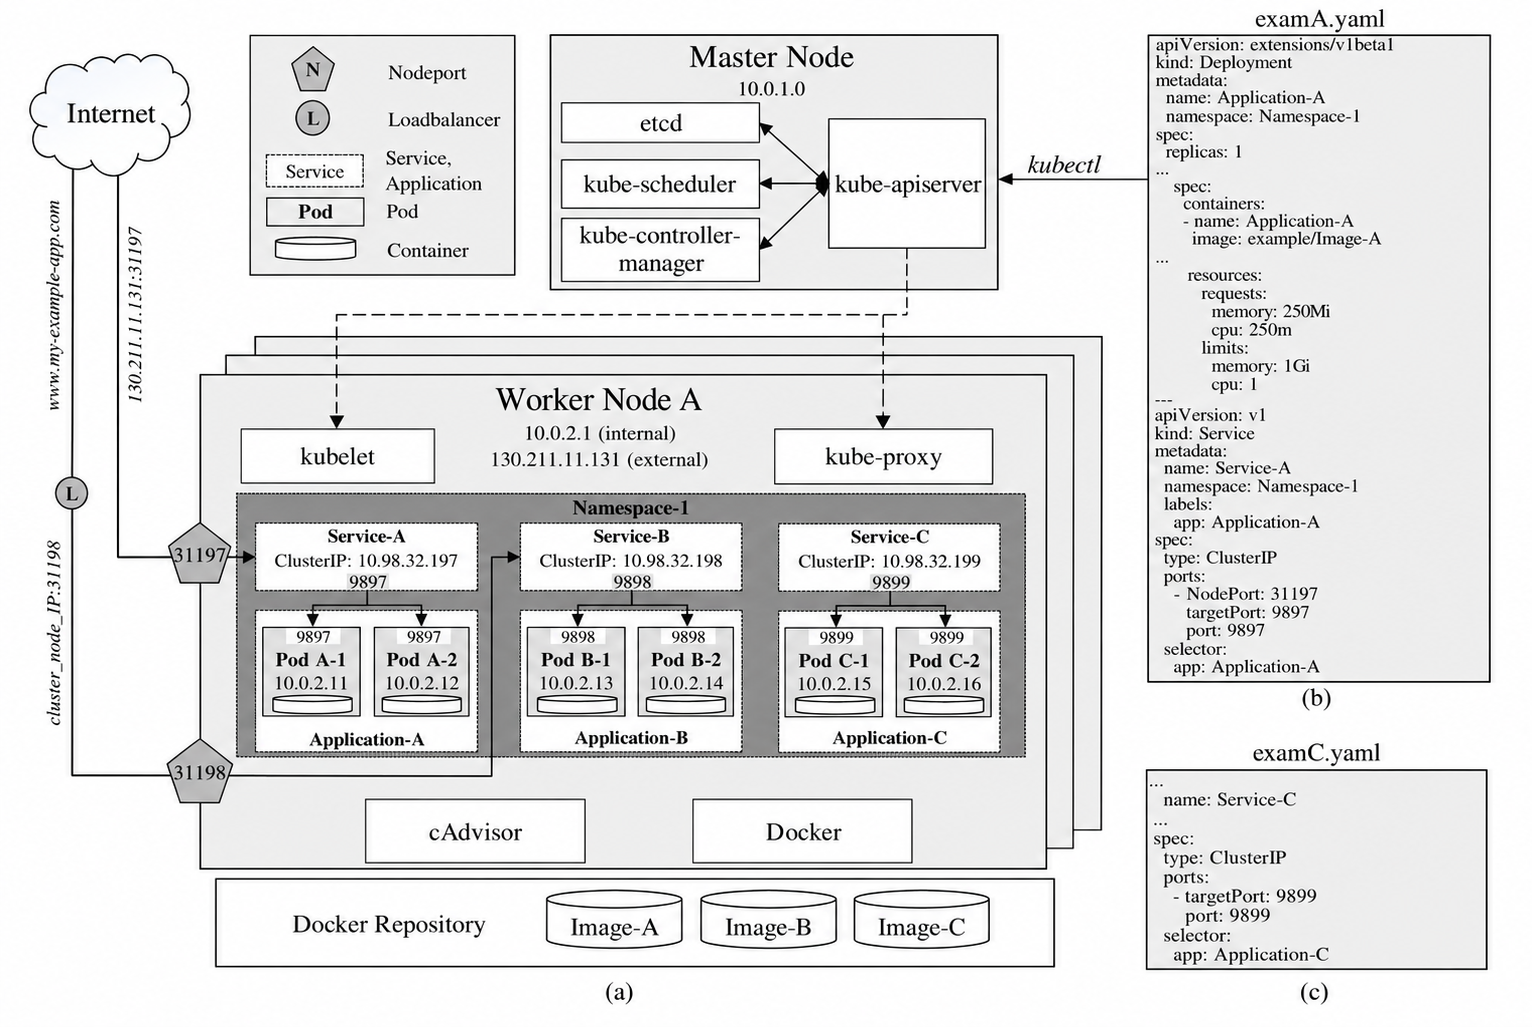
\includegraphics[width=0.85\textwidth]{processed-results-websockets/K8-hpa-architecuture.png}
\caption{Standard Kubernetes HPA feedback loop architecture, reproduced from Nguyen et al.~\cite{nguyen2020hpa}. The HPA controller operates as a discrete-time proportional regulator: it periodically reads aggregated resource metrics from the API server (sourced either from the Metrics Server for KRM or the Prometheus Adapter for PCM) and computes a desired replica count using Equation~\ref{eq:hpa}. A critical architectural constraint is that this loop assumes the observed metric faithfully represents current workload intensity - an assumption that is violated for persistent-connection workloads where connections persist independently of CPU utilization.}
\label{fig:hpa_arch}
\end{figure*}

\subsection{Kubernetes Resource Metrics (KRM) Pipeline}

In the KRM pipeline, CPU and memory consumption are collected by \texttt{cAdvisor} within each node's \texttt{kubelet}, aggregated by the Metrics Server, and exposed to the HPA controller via the \texttt{metrics.k8s.io} API. Our KRM baseline experiment employed a CPU-intensive HTTP workload with square-wave demand cycles (100~s HIGH at 50~req/s; 100~s LOW at 2~req/s) on a 4-node Kind cluster~\cite{kind_docs}. The following behavioral characteristics were observed:

\begin{itemize}[leftmargin=*]
\item \textbf{Staircase scaling:} Replica increments occur in discrete steps synchronized with the HPA evaluation period, producing a characteristic staircase profile in both the CPU (Figure~\ref{fig:krm_cpu}) and replica count signals.
\item \textbf{CPU overshoot:} Observed utilization exceeds 200\% of the requested CPU allocation during burst onset, reflecting the lag between demand growth and replica provisioning.
\item \textbf{Actuation delay:} A measurable divergence between \texttt{desiredReplicas} and \texttt{currentReplicas} persists through pod scheduling and container initialization (Figure~\ref{fig:krm_desired}).
\item \textbf{Stable convergence:} Despite transient deviations, the closed-loop system reaches steady state without oscillatory instability under unimodal load transitions.
\end{itemize}

\begin{figure*}[t]
\centering
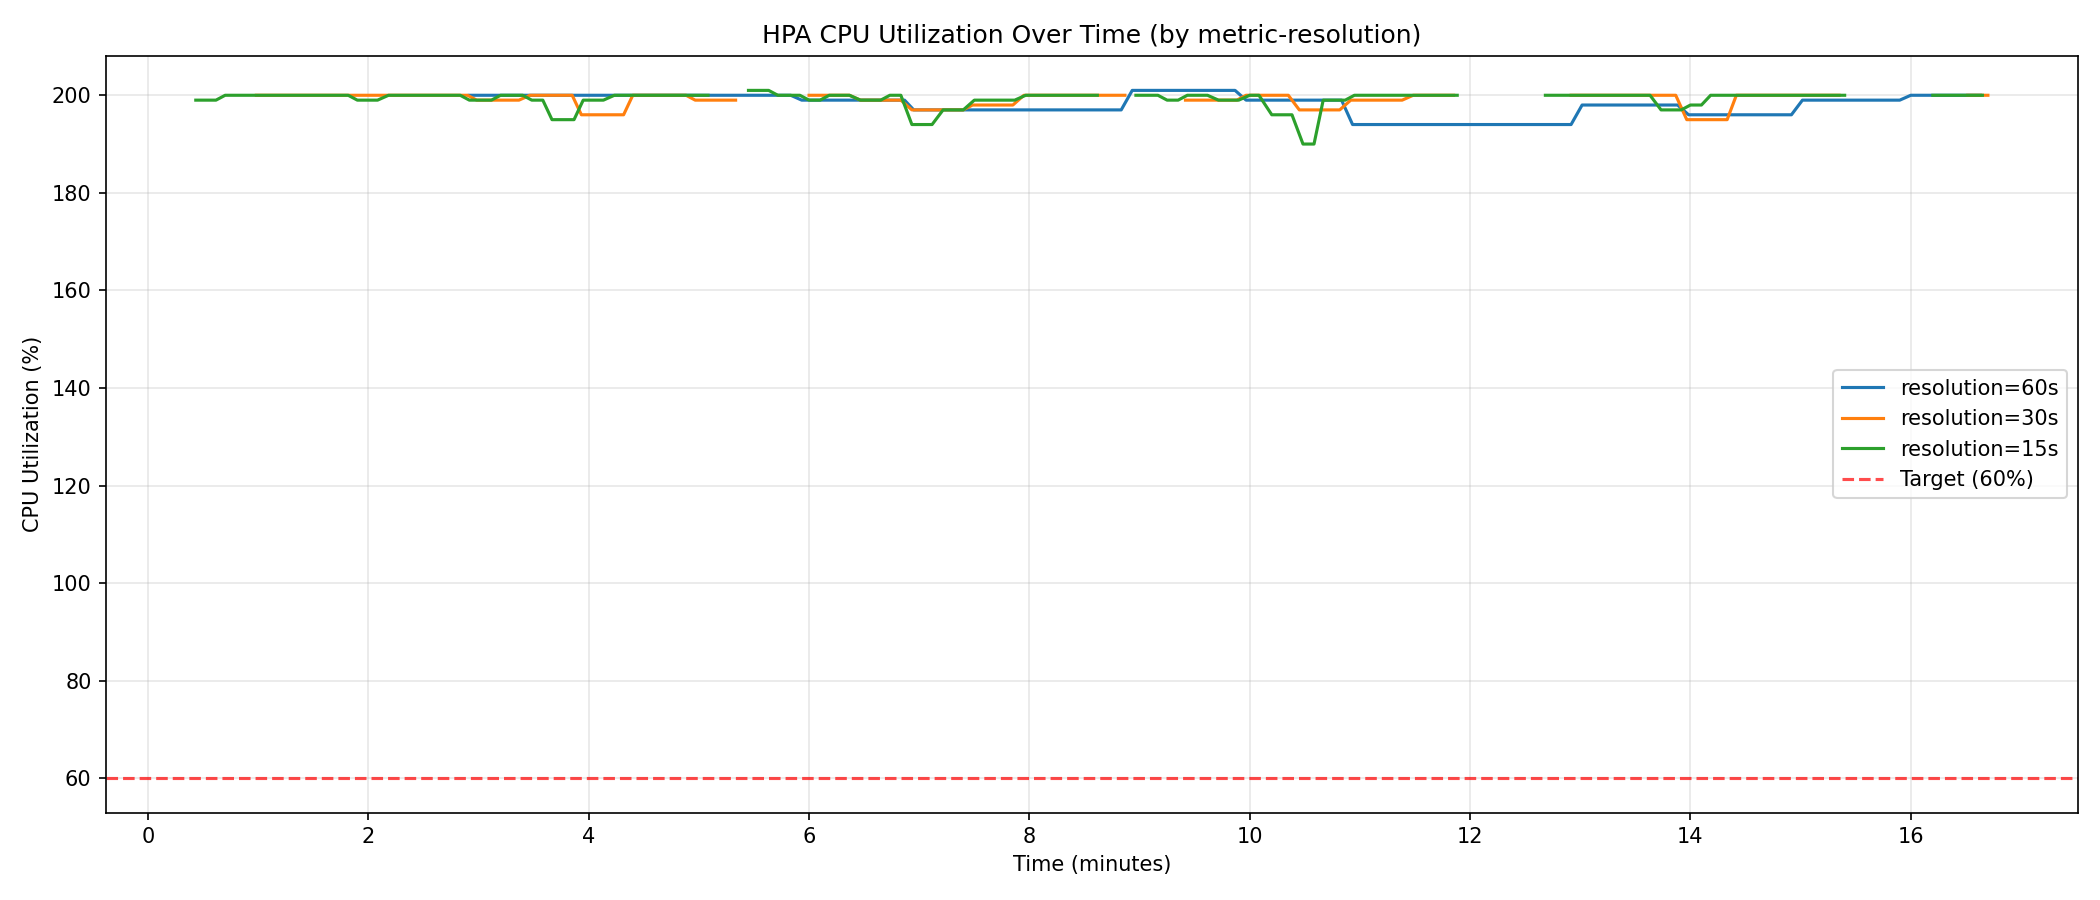
\includegraphics[width=0.85\textwidth]{processed-results-websockets/krm-results/cpu_over_time.png}
\caption{KRM baseline: Observed CPU utilization over time. Significant overshoot above the 60\% target threshold occurs at burst onset, reflecting the inherent actuation delay of the discrete-time proportional control loop.}
\label{fig:krm_cpu}
\end{figure*}

\begin{figure*}[t]
\centering
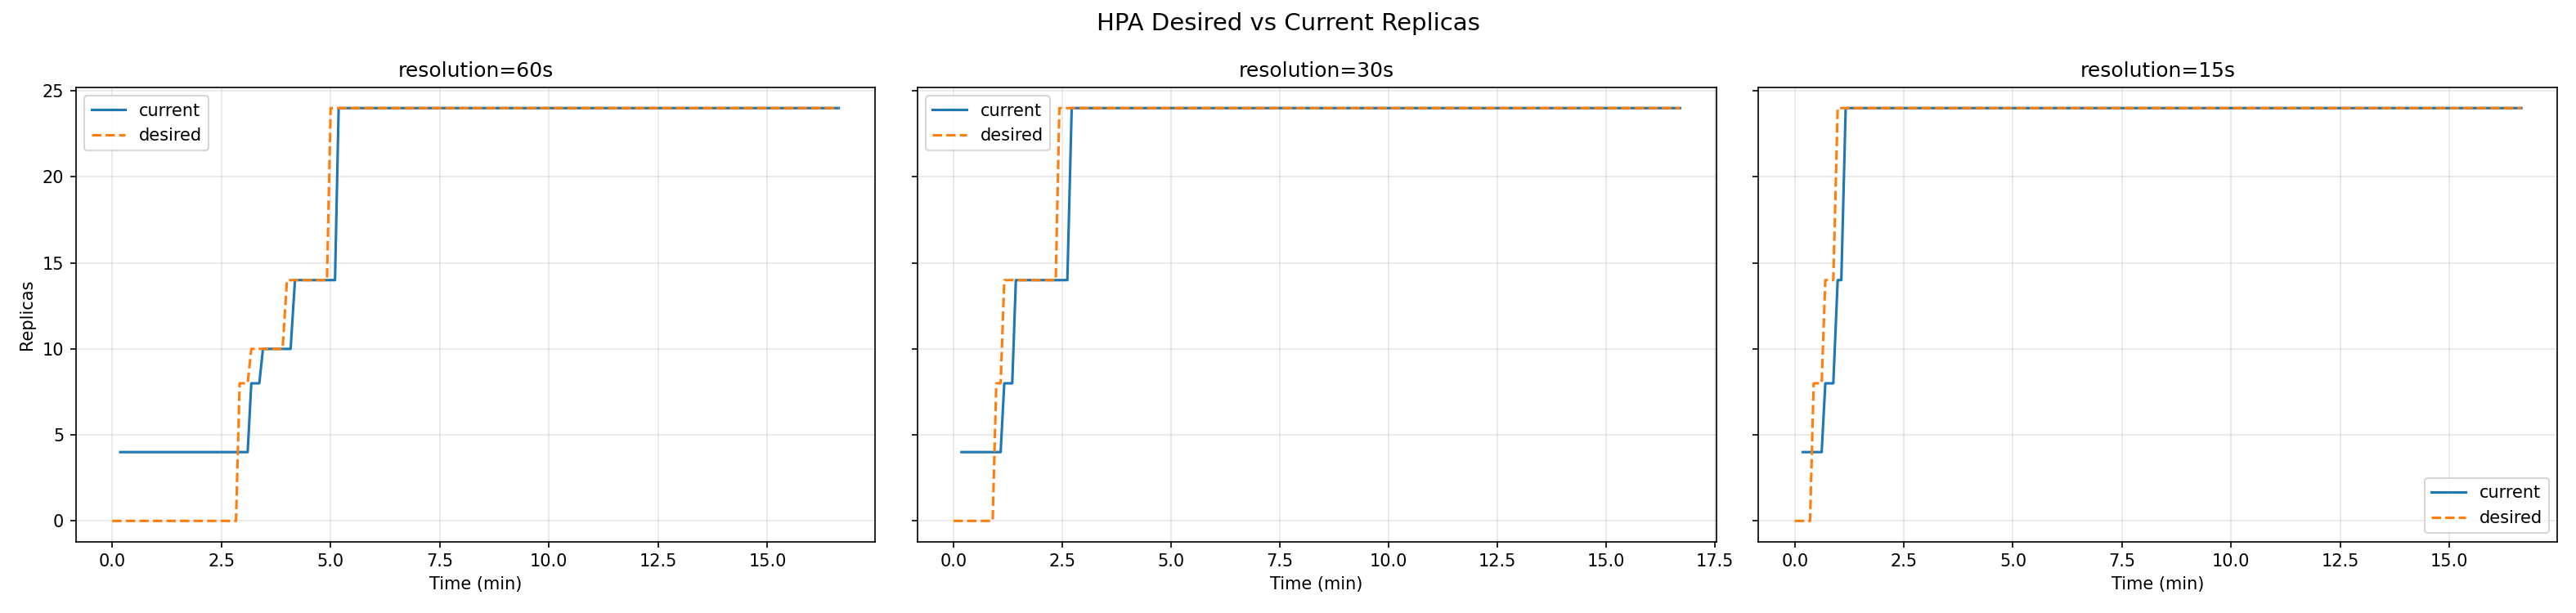
\includegraphics[width=0.85\textwidth]{processed-results-websockets/krm-results/desired_vs_current.png}
\caption{KRM baseline: Divergence between \texttt{desiredReplicas} (as computed by HPA) and \texttt{currentReplicas} (as observed in the deployment) across scale-up events. The gap quantifies the combined actuation delay attributable to pod scheduling latency and container startup time.}
\label{fig:krm_desired}
\end{figure*}

\subsection{Prometheus Custom Metrics (PCM) Pipeline}

The PCM pipeline introduces additional stages: application pods expose Prometheus-format metrics via an HTTP endpoint; the Prometheus server scrapes and stores these as time series; the Prometheus Adapter translates PromQL query results into the Kubernetes Custom Metrics API; and HPA consumes the resulting per-pod values. Following the methodology of Nguyen et al.~\cite{nguyen2020hpa}, we evaluate three PCM configurations and three scrape intervals:

\begin{itemize}[leftmargin=*]
\item \textbf{PCM-CPU:} CPU utilization sourced via Prometheus rather than the Metrics Server.
\item \textbf{PCM-H:} HTTP request rate, providing a demand-leading indicator.
\item \textbf{PCM-CH:} Hybrid combination of CPU utilization and HTTP request rate.
\end{itemize}

\begin{figure*}[t]
\centering
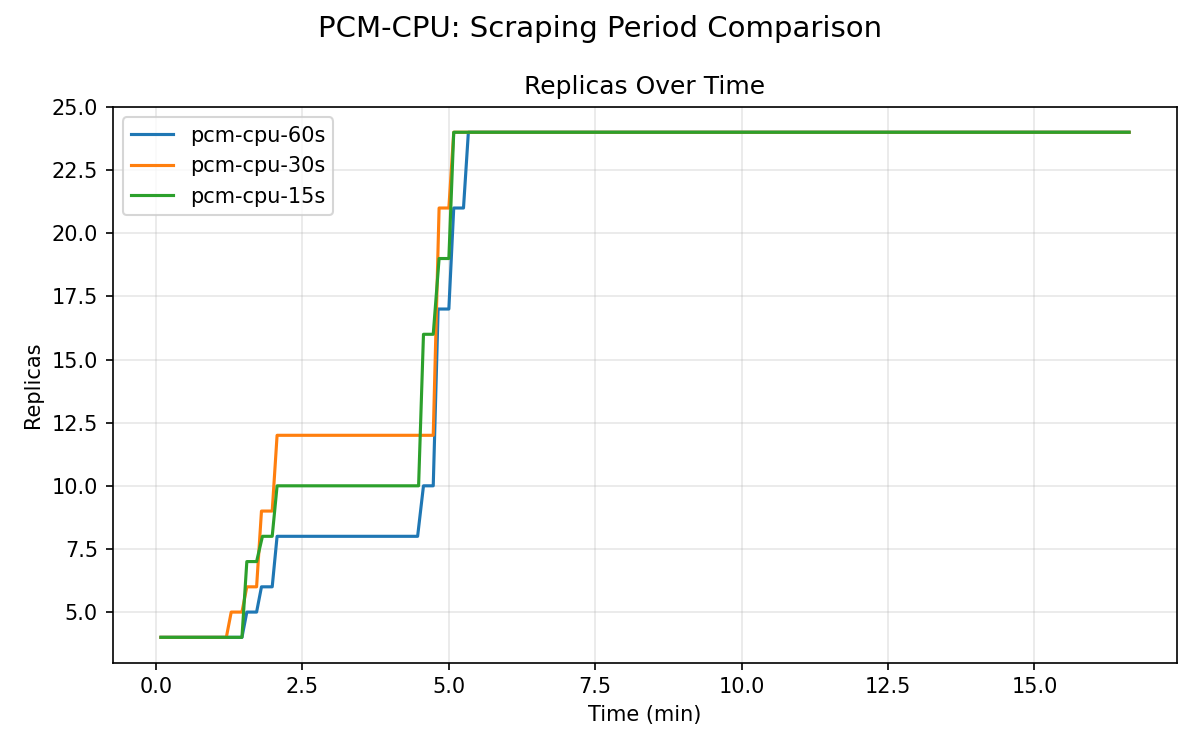
\includegraphics[width=0.85\textwidth]{processed-results-websockets/pcm-results/PCM-scraping_period_comparison.png}
\caption{PCM baseline: Effect of Prometheus scrape interval (15~s, 30~s, 60~s) on HPA scaling responsiveness. A 60~s scrape interval introduces visible staircase delay that significantly degrades scale-up latency; reducing to 30~s yields a substantial improvement, while the marginal gain from 30~s to 15~s is comparatively small - consistent with the findings of Nguyen et al.~\cite{nguyen2020hpa}.}
\label{fig:pcm_scrape}
\end{figure*}

Key findings (Figure~\ref{fig:pcm_scrape}) replicate and extend the analysis in~\cite{nguyen2020hpa}: reducing the scrape interval from 60~s to 30~s materially improves scale-up latency, with diminishing returns at 15~s. PCM-H provides the earliest reaction to demand increases but at the cost of transient over-provisioning; PCM-CH reduces oscillation by combining the leading indicator (request rate) with the stabilizing feedback (CPU).

These baselines confirm that HPA behaves as a well-functioning proportional regulator for stateless workloads in which the chosen metric tracks demand monotonically. The critical experimental question is: \textbf{what are the consequences of this control design when the assumed signal-to-demand coupling is structurally absent?}

\subsection{The HPA Control Architecture}

Figure~\ref{fig:hpa_arch} illustrates the Kubernetes HPA feedback loop as documented by Nguyen et al.~\cite{nguyen2020hpa}. The HPA controller implements the following discrete-time proportional control law evaluated every 15~seconds (the default synchronization period):
\begin{equation}
\textit{desiredReplicas} = \left\lceil \textit{currentReplicas} \times \frac{\textit{currentMetricValue}}{\textit{targetMetricValue}} \right\rceil
\label{eq:hpa}
\end{equation}

This formulation implicitly encodes the assumption that \texttt{currentMetricValue} truthfully reflects the workload intensity across all running replicas. For CPU-based scaling of stateless workloads, this assumption generally holds. For persistent-connection workloads, it fails categorically: idle connections consume negligible CPU yet represent committed session state whose disruption is immediately visible to end clients.


%% ============================================================
\section{Problem: Empirical Evidence of HPA Failure for Stateful WebSocket Workloads}
\label{sec:problem}
%% ============================================================

We present a controlled, progressive chain of experiments designed to isolate and characterize each failure mode of CPU-based HPA when applied to persistent WebSocket workloads. The experiments are ordered from least severe (over-provisioning) to most severe (permanent connection destruction), with each experiment building upon the instrumentation and findings of its predecessor. All WebSocket experiments share a common infrastructure: a 3-node Kind cluster (1 control-plane + 2 worker nodes, Kubernetes v1.31.6, kind v0.25.0, configured via \texttt{kind.yml})~\cite{kind_docs}. The Metrics Server is patched with \texttt{-metric-resolution=15s} and \texttt{-kubelet-insecure-tls} (required for kind's self-signed kubelet certificates; not appropriate for production). All experimental scripts, cluster configuration, server code, load generator, and controller source are available at: \url{https://github.com/AbhasBenevolentDictator/STAR}. Experiments can be reproduced on any Linux machine with Docker and kind installed by running the numbered experiment scripts in \texttt{scripts/}. The shared experimental infrastructure comprises: a custom Python asyncio WebSocket server (image: \texttt{ws-instrumented}), 800 persistent client connections established by the load generator, and Kubernetes HPA configured with \texttt{targetCPUUtilizationPercentage: 60} unless stated otherwise.

\paragraph{Instrumented server: definition and rationale}
By "instrumented" we mean the server was extended to expose Prometheus-format metrics (notably a gauge \texttt{active\_connections} and a counter \texttt{new\_connections\_total}) and a minimal control endpoint (for example, \texttt{/drain}) to enable graceful handoff. We adopted this instrumentation to obtain direct, low-latency visibility into live session counts and connection churn — signals that CPU does not capture. This approach was selected because it (i) supplies a precise scaling signal for the controller, (ii) permits reproducible measurement of reconnection storms via PromQL rate() on \texttt{new\_connections\_total}, and (iii) is minimally invasive and portable (it can be implemented in-application or as a small sidecar/exporter), improving experimental repeatability and external validity.

\subsection{Experiment A: HPA Baseline Under Monotonic Correlated Load}

\paragraph{Hypothesis.} Under steady, monotonically increasing WebSocket load in which each connection actively generates CPU work (\texttt{CPU\_WORK=1}), HPA will correctly scale the deployment, establishing an empirical baseline for comparison with subsequent experiments.

\paragraph{Experimental Setup.} Eight hundred WebSocket clients connect incrementally over 300~seconds. Each server-side message receipt triggers a bounded CPU spin loop, maintaining strict proportionality between active connection count and CPU utilization: CPU $\propto$ connections. HPA was configured with \texttt{minReplicas=2}, \texttt{maxReplicas=10}, and \texttt{targetCPUUtilizationPercentage=60}.

\paragraph{Results.} As shown in Figure~\ref{fig:exp_a_replicas}, HPA scaled the deployment monotonically from 2 to 5 replicas as CPU rose proportionally with connection count. Following complete load removal, the system enforced the default 300-second scale-down stabilization window before descending cleanly to \texttt{minReplicas}. No oscillatory behavior or reconnection disruption was observed.

\begin{figure}[ht]
\centering
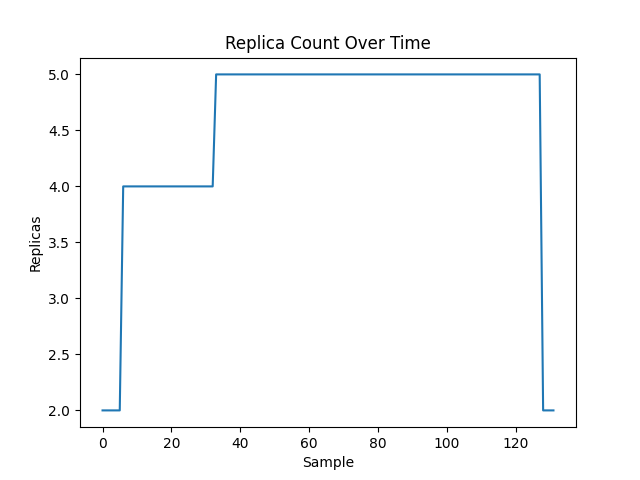
\includegraphics[width=\columnwidth]{processed-results-websockets/experiment-a-hpa/replicas.png}
\caption{Experiment A: Replica count timeline under monotonic WebSocket load with CPU $\propto$ connections. The clean staircase ascent (2$\rightarrow$5), flat stabilization plateau, and controlled descent to the minimum represent the theoretical ideal for HPA - achievable only under perfect signal-to-demand correlation.}
\label{fig:exp_a_replicas}
\end{figure}

The replica timeline (Figure~\ref{fig:exp_a_replicas}) confirms that HPA operates correctly \textit{when its signal accurately encodes workload demand}. Crucially, this experiment represents a best-case scenario that is structurally unachievable in production WebSocket deployments, where connection activity levels are decoupled from CPU consumption.

\begin{keyresult}
\noindent\textbf{Conclusion.} CPU-based HPA functions correctly only under the idealized condition of perfect CPU-to-connection proportionality. Subsequent experiments systematically invalidate this condition.
\end{keyresult}

\subsection{Experiment B1: HPA Under Cyclic Load - Over-Provisioning and Recovery Asymmetry}

\paragraph{Hypothesis.} Under realistic cyclic HIGH/LOW load patterns that simulate natural connection activity fluctuations, HPA will exhibit systematic over-provisioning and asymmetrically slow resource recovery.

\paragraph{Experimental Setup.} Load alternates between HIGH phases (800 connections, active CPU-generating pinging, 60-second duration) and LOW phases (connections held persistently idle, no pinging activity, 30-second duration). Crucially, during LOW phases the 800 client connections remain open; only the periodic ping messages cease, collapsing CPU utilization toward zero while connection state is preserved. Parameters were adjusted to \texttt{maxReplicas=15} to allow unconstrained scale-up. The HPA stabilization window was kept at the Kubernetes default of 300~seconds for scale-down (\texttt{stabilizationWindowSeconds: 300}), intentionally unmodified to evaluate HPA behavior under factory settings for cyclic load. Five consecutive HIGH/LOW cycles (60~s HIGH + 30~s LOW = 90-second period) were run, for a total active cycle phase of 450~seconds, after which the system was observed until HPA converged back to \texttt{minReplicas}.

\paragraph{Results.} During HIGH phases, HPA exhausted \texttt{maxReplicas=15} within 99~seconds - a factor of 1.875$\times$ the theoretically correct value of 8~replicas ($\lceil800/100\rceil$). The core mechanism driving over-provisioning is the interaction between the 90-second cycle period and the 300-second stabilization window: each LOW phase (30~s) ends before the window has elapsed, so every new HIGH phase begins with the replica count still at or near the ceiling from the previous cycle. Over five cycles, the replica count ratchets to \texttt{maxReplicas} and remains there, with each brief LOW phase failing to provide enough sustained low-CPU time for HPA to authorize a descent. Convergence to \texttt{minReplicas} following the final cycle required approximately 650~seconds - consistent with the 300-second stabilization window plus the time for graduated scale-down steps. The replica count timeline (Figure~\ref{fig:exp_b1_replicas}) exhibits the expected oscillation pattern between the replica ceiling and floor.

\begin{figure}[ht]
\centering

\includegraphics[width=\columnwidth]{processed-results-websockets/experiment-b1-hpa-churn/replicas.png}
\caption{Experiment B1: HPA saturates at \texttt{maxReplicas=15} within 99~seconds under cyclic load, representing an 87.5\% over-provision relative to the connection-derived optimum. Recovery to the minimum requires $\sim$650~seconds, demonstrating severe asymmetry between scale-up and scale-down responsiveness.}
\label{fig:exp_b1_replicas}
\end{figure}

\begin{keyresult}
\noindent\textbf{Conclusion.} Cyclic workloads expose HPA's inability to distinguish connection-holding periods (where CPU is low but capacity is required) from genuinely idle periods (where capacity can be safely released). The 87.5\% over-provisioning rate and disproportionate recovery time represent significant resource efficiency penalties in production deployments.
\end{keyresult}

\subsection{Experiment B2-Instrumented: Quantifying Reconnection Storm Intensity}

\paragraph{Methodological note: supersession of a non-instrumented pilot}
Prior to this experiment, a preliminary non-instrumented variant (B2-Extended LOW) was conducted in which the LOW phase was extended beyond the default 300-second stabilization window to force HPA all the way to \texttt{minReplicas=2}. While this pilot confirmed that active connections were being severed during scale-down events through qualitative observation of client disconnects, it produced no quantitative data: the server exposed no Prometheus metrics, connection loss counts were unverifiable, and reconnection rates were entirely unobservable. The pilot served its intended engineering purpose - confirming the failure mode was reproducible before investing in full instrumentation - but it contributes no independent publishable evidence beyond what B2-Instrumented already provides with greater precision and statistical depth. Accordingly, B2-Extended LOW is not reported as a standalone experiment in this paper. Its sole scientific contribution is as the direct motivation for adding the Prometheus instrumentation described below.

\paragraph{Hypothesis.} Each HPA scale-down event, by terminating pods hosting active connections, will trigger a measurable reconnection storm with peak rates exceeding 1,000~connections/second, and will induce overshoot of the steady-state connection target due to the cascade of concurrent reconnection attempts.

\paragraph{Experimental Setup.} The WebSocket server was instrumented with two Prometheus metrics: \texttt{active\_connections} (a gauge reflecting current session count) and \texttt{new\_connections\_total} (a monotonically increasing counter enabling rate computation via \texttt{rate()}). Prometheus was configured to scrape at a 15-second interval. The HPA policy was configured with \texttt{stabilizationWindowSeconds: 0} for scale-up, enabling HPA to react immediately to rising CPU without any hysteresis, and \texttt{stabilizationWindowSeconds: 60} for scale-down. Setting scale-up to zero is deliberate: it ensures that each reconnection storm (which spikes CPU) immediately triggers scale-up, guaranteeing that every cycle produces a complete and observable scale-up/scale-down sequence within the measurement window. Each cycle consisted of a 60-second HIGH phase (800 pinging clients, \texttt{CPU\_WORK=1}) followed by a 90-second LOW phase (connections idle, no pinging, \texttt{CPU\_WORK=1} still set but no messages arriving so CPU collapses). The 90-second LOW duration was specifically chosen to exceed the 60-second scale-down stabilization window, ensuring that HPA always executes at least one scale-down event per cycle. Five complete HIGH/LOW cycles were executed to provide statistical repeatability.

\paragraph{Results.} Every HPA scale-down event across all five cycles triggered a distinct, measurable reconnection storm. Storm rates were highly consistent: Cycle 1: 1,400.9~conn/s; Cycle 2: 1,298.3~conn/s; Cycle 3: 1,399.5~conn/s; Cycle 4: 1,251.8~conn/s; Cycle 5 trailed as the connection population had partially degraded by the final cycle. The peak reconnection rate reached \textbf{1,400 connections/second}, as shown in Figure~\ref{fig:exp_b2_reconnections}. Concurrent with each storm, the active connection count transiently overshot the 800-connection steady-state target, peaking at \textbf{1,215 connections} - a 51.9\% overshoot (Figure~\ref{fig:exp_b2_connections}). The socket-level mechanism driving this overshoot is as follows: when a pod is sent \texttt{SIGKILL} after its 30-second termination grace period, its TCP connections are abruptly reset (TCP RST). All 800 clients detect closure simultaneously and immediately initiate reconnection. The Prometheus gauge \texttt{active\_connections} on the surviving pods begins counting new incoming connections before the OS completes cleanup of socket state (including the TIME\_WAIT window for recently reset connections), transiently reporting a total above the 800-client ceiling. The overshoot resolves within 15-30~seconds as OS-level socket reclaim completes.

\begin{figure}[ht]
\centering
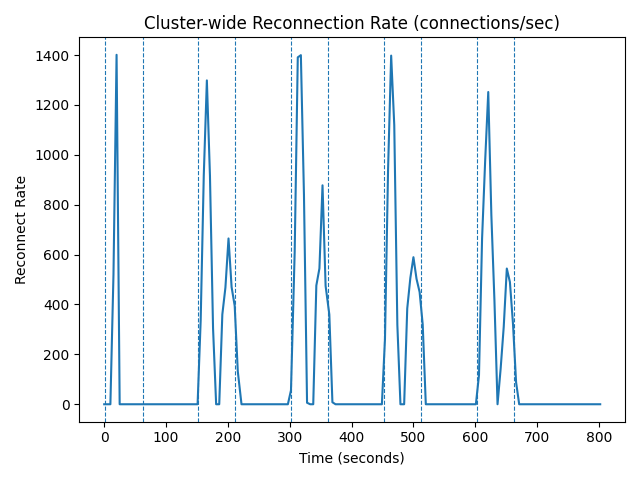
\includegraphics[width=\columnwidth]{processed-results-websockets/experiment-b2-hpa-churn-instrumented/reconnections.png}
\caption{Experiment B2-Instrumented: Prometheus-measured reconnection rate (\texttt{rate(new\_connections\_total[15s])}) over the five-cycle experiment. Each reconnection spike is precisely synchronized with an HPA scale-down event, with peak observed rates of 1,400~connections/second.}
\label{fig:exp_b2_reconnections}
\end{figure}

\begin{figure}[ht]
\centering

\includegraphics[width=\columnwidth]{processed-results-websockets/experiment-b2-hpa-churn-instrumented/connections.png}
\caption{Experiment B2-Instrumented: Active connection count during the reconnection storm period. The connection overshoot of 1,215 (51.9\% above the 800-client target) arises as reconnecting clients establish new sessions before the server has fully released the state associated with severed connections.}
\label{fig:exp_b2_connections}
\end{figure}

Figure~\ref{fig:exp_b2_scaling} provides the combined view of replica oscillation and connection disruption, establishing the causal chain from HPA scaling decision to client-side session disruption.

\begin{figure}[ht]
\centering
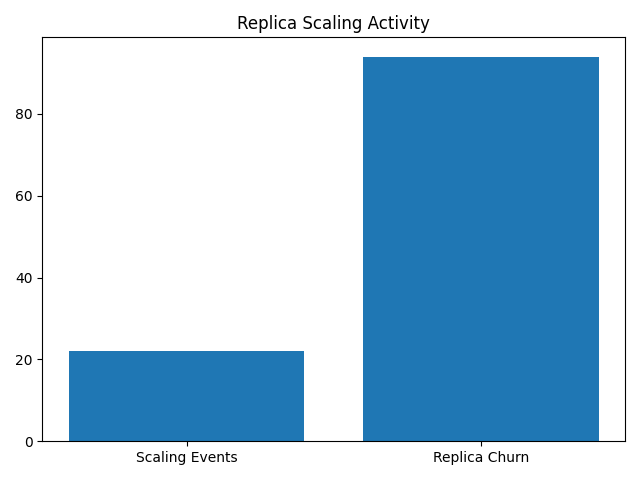
\includegraphics[width=\columnwidth]{processed-results-websockets/experiment-b2-hpa-churn-instrumented/scaling_activity.png}
\caption{Experiment B2-Instrumented: Temporal correlation between HPA replica changes (green) and active connection count (blue). Each downward step in replicas corresponds to a measurable spike in the connection disruption signal, confirming the direct causal relationship.}
\label{fig:exp_b2_scaling}
\end{figure}

\begin{keyresult}
\noindent\textbf{Conclusion.} HPA scale-down events are inherently destructive to WebSocket client sessions. Each replica reduction simultaneously severs all connections hosted on the terminated pod, producing a reconnection storm whose intensity scales with the connection density of the removed replica. At 1,400~conn/s, such storms represent a severe degradation event for latency-sensitive applications.
\end{keyresult}

\subsection{Experiment B3: Permanent Connection Loss Under Non-Reconnecting Clients}

\paragraph{Hypothesis.} When WebSocket clients do not implement reconnection logic - modeling clients that treat connection loss as a terminal failure (e.g., batch data collectors, embedded IoT sensors, or long-running streaming sessions) - HPA scale-down events will cause \textit{permanent, irrecoverable reduction} in the total session population.

\paragraph{Experimental Setup.} The load generator was reconfigured with \texttt{reconnect: false}. Once a client's connection is severed by pod termination, the client neither retries nor reconnects. The HPA policy mirrored B2-Instrumented: \texttt{stabilizationWindowSeconds: 0} for scale-up (fast reaction to pinging activity) and \texttt{stabilizationWindowSeconds: 60} for scale-down. CPU work was retained (\texttt{CPU\_WORK=1}) to maintain HPA activity, but the metric of interest is the cumulative active connection count. The IDLE phase runs for up to 240~seconds (\texttt{IDLE\_MAX\_DURATION=240}), providing sufficient headroom for HPA to execute multiple sequential scale-down events within a single experiment run.

\paragraph{Pod termination mechanics and the 30-second limbo}
Understanding the exact Kubernetes pod termination sequence is essential for interpreting this experiment's figures. When HPA reduces \texttt{spec.replicas}, the following steps occur in order: (1)~the target pod is immediately removed from the Service's endpoint slice, so no new connections are routed to it; (2)~Kubernetes sends \texttt{SIGTERM} to the pod's main process and starts the \texttt{terminationGracePeriodSeconds} timer (default: 30~s); (3)~during the 30-second grace period, existing TCP connections on the terminating pod remain open and functional - they are maintained by the OS kernel, not Kubernetes - and the pod continues to service those connections; (4)~after \texttt{terminationGracePeriodSeconds} elapses, Kubernetes sends \texttt{SIGKILL}, which tears down the process and the OS forcibly resets all open TCP connections (TCP RST). This sequence is why the active connection drop visible in Figure~\ref{fig:exp_b3_connections} lags behind HPA's scale-down decision by approximately 30~seconds: the connection is not immediately destroyed when HPA acts, but is destroyed 30~seconds later when \texttt{SIGKILL} fires. This delay does not mitigate the harm - the connection still dies, the client still receives a TCP RST, and with \texttt{reconnect: false}, the session is permanently lost.

\paragraph{Results.} The active connection count (Figure~\ref{fig:exp_b3_connections}) exhibits a characteristic \textbf{staircase step-down} pattern. Each step corresponds precisely to an HPA scale-down decision: when a pod is terminated, the full contents of its connection table are permanently destroyed. Successive scale-down events cause monotonically fewer active connections, with no mechanism for recovery.

\begin{figure*}[t]
\centering

\includegraphics[width=0.85\textwidth]{processed-results-websockets/experiment-b3-hpa-idle-connections/connections.png}
\caption{Experiment B3: Active connection count exhibits permanent staircase destruction (800$\rightarrow$744$\rightarrow$697$\rightarrow$445$\rightarrow$79). Each step-down is precisely synchronized with an HPA scale-down event. The connections are irrecoverable under the \texttt{reconnect: false} regimen.}
\label{fig:exp_b3_connections}
\end{figure*}

The combined view in Figure~\ref{fig:exp_b3_combined} provides the definitive causal chain: (1)~connections become idle and cease to generate CPU load; (2)~HPA, observing near-zero CPU, decides to scale down; (3)~the terminated pod destroys all connections it hosts permanently. This is not a failure of any particular configuration parameter - it is an architectural failure arising from HPA's inability to observe connection state as a first-class scaling signal.

\begin{figure*}[t]
\centering
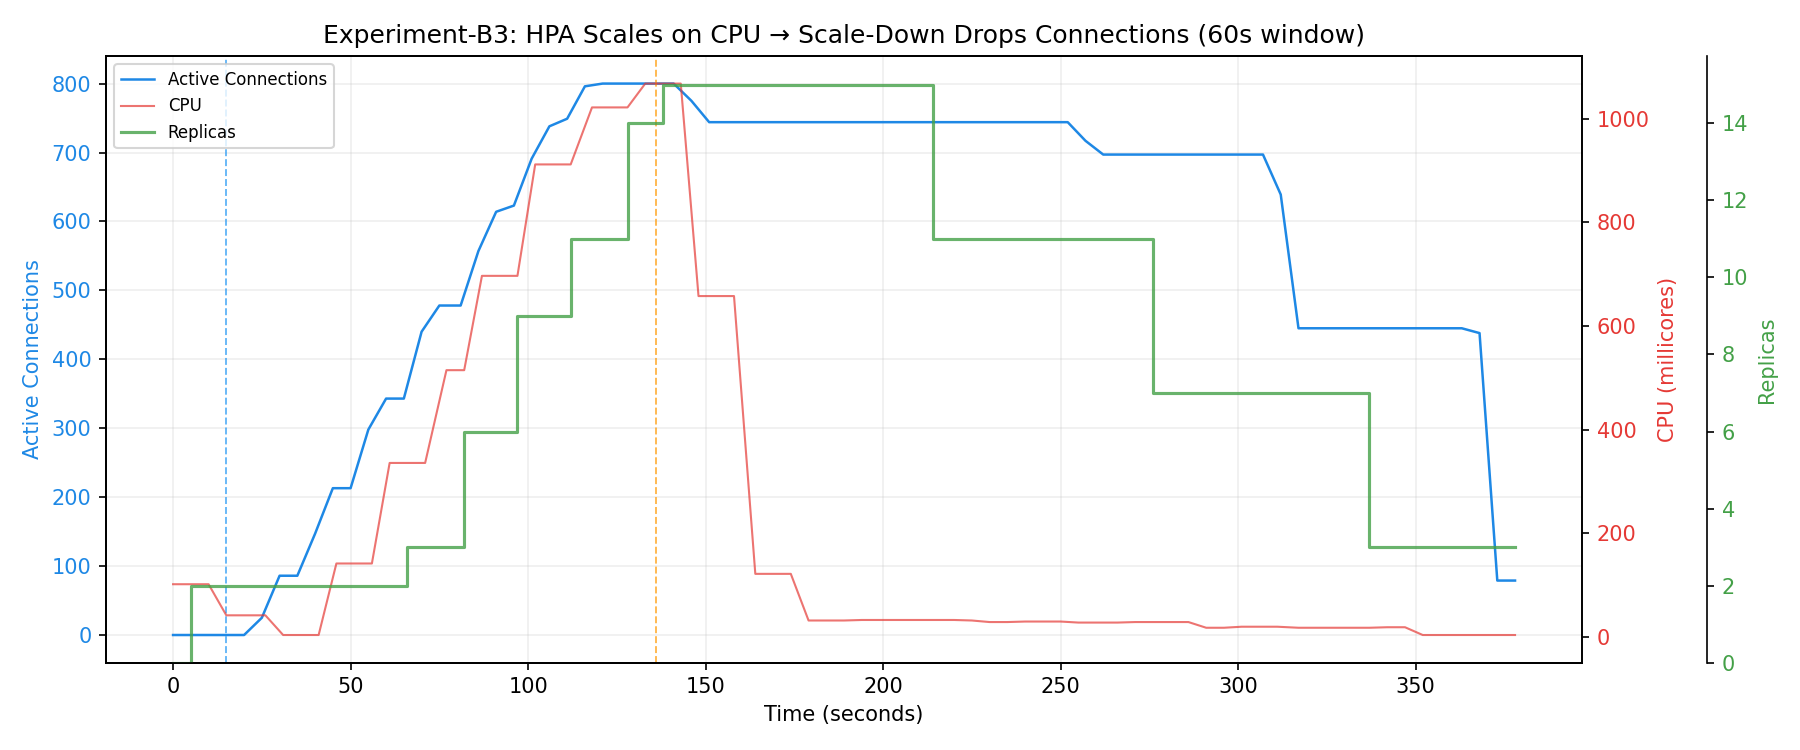
\includegraphics[width=0.85\textwidth]{processed-results-websockets/experiment-b3-hpa-idle-connections/combined.png}
\caption{Experiment B3, combined signal view - the causal proof of the mismatch between CPU-based scaling signals and stateful workload characteristics. CPU utilization (red) drops to near zero as connections become idle $\rightarrow$ HPA scales down the replica count (green) $\rightarrow$ active connections (blue) are permanently destroyed. The autoscaler is induced by its own metric to destroy the session state it should be protecting.}
\label{fig:exp_b3_combined}
\end{figure*}

\begin{keyresult}
\noindent\textbf{Conclusion.} The exclusive reliance of HPA on CPU as a scaling signal causes the autoscaler to be structurally antagonistic to idle-but-connected stateful workloads. This finding demonstrates that the problem cannot be remediated by parameter tuning; it requires a fundamentally different scaling architecture.
\end{keyresult}

\subsection{Summary of the Evidence Chain}

Table~\ref{tab:failure_summary} consolidates the progressive evidence across all four HPA experiments.

\begin{table*}[t]
\centering
\caption{Summary of the progressive evidence chain demonstrating the failure of CPU-based HPA for stateful WebSocket workloads. Each experiment isolates and quantifies a distinct failure mode.}
\label{tab:failure_summary}
\begin{tabular}{@{}p{2.2cm}p{3.5cm}p{3.5cm}p{5cm}@{}}
\toprule
\rowcolor{gray!12}
\textbf{Experiment} & \textbf{Condition} & \textbf{HPA Behavior} & \textbf{Key Quantitative Finding} \\
\midrule
A (Baseline) & Monotonic load; CPU $\propto$ connections & Correct proportional scaling & Works only under idealized signal correlation \\
B1 (Cyclic) & Alternating HIGH/LOW activity & Reaches \texttt{maxReplicas} in 99~s & 87.5\% over-provisioning; 650~s to recover \\
B2-Inst. (Measured) & Cyclic + Prometheus instrumentation & Reconnection storm per scale-down & Peak 1,400~conn/s; 51.9\% connection overshoot \\
B3 (No-reconnect) & Idle connections; no client retry & Permanent, staircase connection loss & 800$\rightarrow$79 active connections; zero recovery \\
\bottomrule
\end{tabular}
\end{table*}


%% ============================================================
\section{Proposed Solution: The \texttt{StatefulAutoscaler} Controller}
\label{sec:controller}
%% ============================================================

The failure evidence in Section~\ref{sec:problem} identifies three root causes that any viable solution must address: (1)~the scaling signal (CPU) does not encode the workload state that must be protected; (2)~scale-down decisions are made without knowledge of whether connections are alive; and (3)~no stabilization mechanism exists that is aware of connection-level context. We address all three by designing the \texttt{StatefulAutoscaler}, a custom Kubernetes controller that replaces the CPU-based control loop with a connection-density-based one augmented by connection-context stabilization.

\subsection{Design Principles}

The controller is grounded in three architectural principles:

\begin{enumerate}[leftmargin=*]
\item \textbf{Use the correct scaling signal.} The controller queries \texttt{sum(active\_connections)} from Prometheus - the metric that directly encodes the workload state that must be preserved. CPU is never consulted.

\item \textbf{Compute replica counts from connection density.} Given a configured target of $T$ connections per pod, the desired replica count is:
\begin{equation}
\textit{desiredReplicas} = \left\lceil \frac{\texttt{sum(active\_connections)}}{T} \right\rceil
\label{eq:stateful}
\end{equation}
This formulation is exact by construction: it scales the system to exactly the minimum number of replicas required to serve the current session population at the target density.

\item \textbf{Stabilize scale-down decisions using connection-context history.} A sliding-window mechanism maintains the maximum desired replica count observed within the preceding $N$ seconds, preventing premature scale-down during transient connection drops - the key operational scenario that HPA cannot handle.
\end{enumerate}

\subsection{Custom Resource Definition}

The controller introduces a \texttt{StatefulAutoscaler} Custom Resource Definition (CRD) under the API group \texttt{autoscaling.star.local/v1alpha1}. Table~\ref{tab:crd} documents the key specification fields.

\begin{table}[ht]
\centering
\caption{\texttt{StatefulAutoscaler} CRD specification: key fields and their operational purpose.}
\label{tab:crd}
\begin{tabular}{@{}lp{4.6cm}@{}}
\toprule
\rowcolor{gray!12}
\textbf{Field} & \textbf{Operational Purpose} \\
\midrule
\texttt{targetRef} & Reference to the controlled Deployment \\
\texttt{minReplicas} & Minimum allowable replica count (floor) \\
\texttt{maxReplicas} & Maximum allowable replica count (ceiling) \\
\texttt{targetConnsPerPod} & Connection density target $T$ (Equation~\ref{eq:stateful}) \\
\texttt{maxScaleUpStep} & Maximum replica additions per reconciliation cycle \\
\texttt{maxScaleDownStep} & Maximum replica removals per reconciliation cycle \\
\texttt{scaleDownCooldownSec} & Duration of the sliding stabilization window (seconds) \\
\bottomrule
\end{tabular}
\end{table}

\subsection{System Architecture Overview}

Figure~\ref{fig:system_arch} illustrates the end-to-end system architecture of the \texttt{StatefulAutoscaler} within a Kubernetes cluster, showing the complete data and control flow from client connections through to scaling decisions. The architecture comprises five numbered stages: (1)~persistent WebSocket clients connect through the Kubernetes Service (a stable virtual IP) and are distributed across the pod replicas of the target Deployment; (2)~each pod exposes a Prometheus-format \texttt{/metrics} endpoint reporting an \texttt{active\_connections} gauge, which the Prometheus server scrapes at a configurable interval; (3)~the \texttt{StatefulAutoscaler Controller Manager} queries Prometheus for the aggregated \texttt{sum(active\_connections)} across all pods; (4)~the controller reads its operational parameters (target connections per pod, cooldown duration, step-size limits) from the \texttt{StatefulAutoscaler} Custom Resource (CR), an instance of the CRD defined in Table~\ref{tab:crd}; and (5)~based on the computed desired replica count, the controller patches \texttt{Deployment.spec.replicas} to effect scale-up or scale-down. A critical architectural property, emphasised in the diagram's legend, is that CPU is explicitly excluded from the control path - the entire feedback loop operates on connection density alone. The accompanying CRD example in Figure~\ref{fig:system_arch} shows a representative \texttt{StatefulAutoscaler} manifest with all configurable fields, providing operators with a concrete deployment reference.

\begin{figure*}[t]
\centering
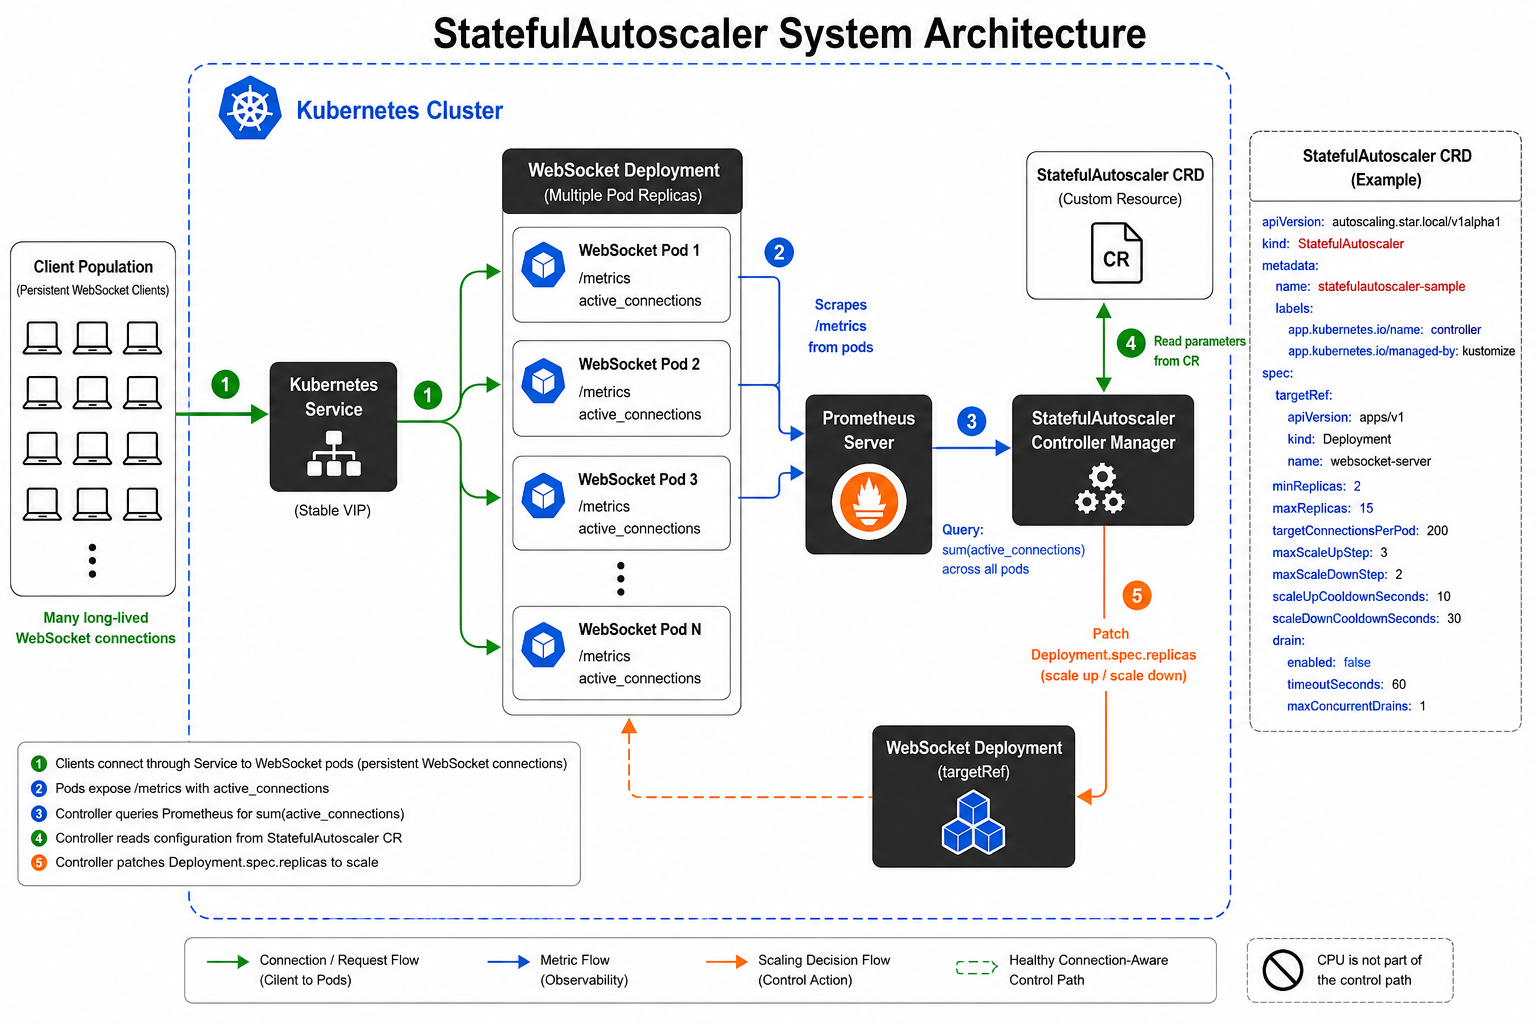
\includegraphics[width=0.95\textwidth]{processed-results-websockets/StatefulAutoScaler-System_Architecture-CRD.png}
\caption{\texttt{StatefulAutoscaler} system architecture and CRD example. The numbered flow shows: (1)~clients connect through the Kubernetes Service to WebSocket pods; (2)~pods expose \texttt{active\_connections} via Prometheus \texttt{/metrics} endpoints; (3)~the controller queries Prometheus for \texttt{sum(active\_connections)}; (4)~operational parameters are read from the \texttt{StatefulAutoscaler} Custom Resource; (5)~the controller patches \texttt{Deployment.spec.replicas} to scale. CPU is explicitly excluded from the control path (crossed-out icon in the legend). The right panel shows a representative CRD manifest with all configurable fields from Table~\ref{tab:crd}.}
\label{fig:system_arch}
\end{figure*}

\subsection{Reconciliation Loop Design}

The controller executes a reconciliation loop every 5~seconds. Algorithm~\ref{alg:reconcile} presents the complete logic, with particular attention to the stabilization window mechanism (lines 7-9) which is the primary differentiating mechanism relative to HPA.

\begin{algorithm}[ht]
\caption{\texttt{StatefulAutoscaler} Reconciliation Logic}
\label{alg:reconcile}
\begin{algorithmic}[1]
\Require StatefulAutoscaler resource $S$, target Deployment $D$
\State $C \gets$ \Call{QueryPrometheus}{\texttt{sum(active\_connections)}}
\If{$C$ is unavailable}
    \State \textbf{requeue} after 10~s \Comment{Conservative default: take no action on missing data}
    \State \Return
\EndIf
\State $raw \gets \lceil C\ /\ S.\texttt{targetConnsPerPod} \rceil$
\State $raw \gets \text{clamp}(raw,\ S.\texttt{minReplicas},\ S.\texttt{maxReplicas})$
\State $W.\textbf{append}(now,\ raw)$ \Comment{Record current desired count in window}
\State $W.\textbf{evict}(\text{entries older than } S.\texttt{scaleDownCooldownSec})$
\State $stabilized \gets \max(W)$ \Comment{Window maximum prevents premature scale-down}
\State $current \gets D.\texttt{spec.replicas}$
\If{$stabilized > current$}
    \State $target \gets \min(current + S.\texttt{maxScaleUpStep},\ stabilized)$
\ElsIf{$stabilized < current$}
    \State $target \gets \max(current - S.\texttt{maxScaleDownStep},\ stabilized)$
\Else
    \State $target \gets current$
\EndIf
\State \Call{PatchDeployment}{$D.\texttt{spec.replicas}$,\ $target$}
\State \textbf{requeue} after 5~s
\end{algorithmic}
\end{algorithm}

Figure~\ref{fig:reconcile_uml} provides a UML activity diagram that visualises the complete reconciliation flow of Algorithm~\ref{alg:reconcile}. The diagram traces the control path from the initial read of the \texttt{StatefulAutoscaler} resource through to the final requeue, making three aspects of the design visually explicit. First, the Prometheus query failure branch (right side) shows the conservative safe-default: when metric data is unavailable, the controller takes no scaling action and requeues after 10~seconds, ensuring that transient observability outages never trigger destructive scale-down decisions. Second, the central vertical path illustrates the key stabilization mechanism: after computing and clamping the raw desired replica count, the controller appends the value to the sliding window history, evicts entries older than \texttt{scaleDownCooldownSeconds}, and derives the stabilized count as the window maximum - preserving the high-water mark of recent connection demand. The annotation in the diagram highlights this as the mechanism that preserves warm pods through transient connection drops. Third, the three-way branching at the bottom shows how the stabilized value is compared against the current replica count to determine whether to scale up (bounded by \texttt{maxScaleUpStep}), scale down (bounded by \texttt{maxScaleDownStep}), or hold steady. All three paths converge at the deployment patch and 5-second requeue, ensuring a continuous feedback loop.

\begin{figure}[ht]
\centering
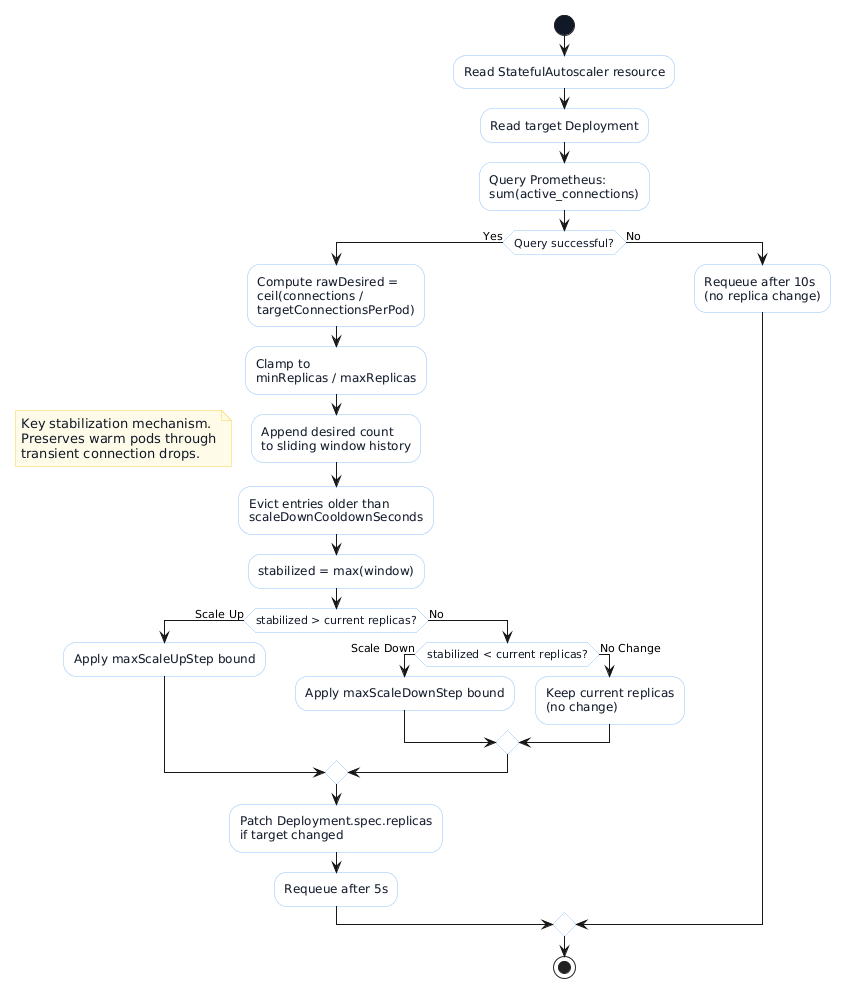
\includegraphics[width=\columnwidth]{processed-results-websockets/StatefulAutoscaler Reconciliation Flow-UML.png}
\caption{UML activity diagram of the \texttt{StatefulAutoscaler} reconciliation loop (Algorithm~\ref{alg:reconcile}). The flow begins with reading the CR and target Deployment, queries Prometheus for \texttt{sum(active\_connections)}, and branches on query success. The central path computes the clamped desired count, updates the sliding window, and derives the stabilized replica target via \texttt{max(window)}. The three-way comparison against current replicas applies step-size bounds before patching the Deployment. The safe-default branch (right) ensures no scaling action is taken when metrics are unavailable.}
\label{fig:reconcile_uml}
\end{figure}

\subsection{The Stabilization Window: Mechanism and Correctness}

The sliding window maximum (line~9 of Algorithm~\ref{alg:reconcile}) is the mechanism responsible for restorm resilience. Its correctness can be understood by contrasting behavior with and without stabilization.

\textbf{Without stabilization:} If all 800 clients disconnect simultaneously due to a transient network partition or upstream load balancer reconfiguration, the controller computes $\lceil 0/100 \rceil = 0$, clamped to \texttt{minReplicas=2}. It scales from 8 to 2 replicas. When clients reconnect 30~seconds later, the controller must scale from 2 back to 8 - recreating the same provisioning lag and potential reconnection cascade that characterized HPA.

\textbf{With a 120-second stabilization window:} When connections drop to zero, the controller appends $raw=2$ to the window, but the window also contains $desired=8$ entries from the preceding 120~seconds. The stabilized value $\max(W)=8$ overrides the instantaneous computation, and all 8~pods are held warm. When clients reconnect within the window duration, they land on pre-provisioned pods with zero provisioning delay.

A critical distinction from HPA's built-in stabilization window is warranted. HPA's stabilization window operates on \textit{metric signal recommendations}: it buffers computed replica counts derived from CPU observations. Given persistent near-zero CPU (as occurs for idle connections), the window stabilizes a recommendation of \texttt{minReplicas} - still resulting in scale-down. The \texttt{StatefulAutoscaler}'s window stabilizes \textit{connection-derived desired replica counts}, which correctly reflect the last known connection demand. This distinction means that the problem cannot be solved by simply tuning HPA's stabilization window to a longer duration.

\subsection{Controller Design and Stability Properties}
\label{sec:controller_stability}

\paragraph{Feedback loop framing.}
The \texttt{StatefulAutoscaler} implements a discrete-time proportional controller with hysteresis. The control loop at every reconciliation cycle performs three steps:
\begin{enumerate}[leftmargin=*]
\item \textbf{Observe:} $C \gets \texttt{sum(active\_connections)}$ via Prometheus.
\item \textbf{Compare:} $desired = \lceil C / T \rceil$, clamped to $[\texttt{minReplicas},\ \texttt{maxReplicas}]$.
\item \textbf{Act:} If $stabilized \neq current$: patch \texttt{deployment.spec.replicas}.
\end{enumerate}
This mirrors the proportional structure of HPA (Equation~\ref{eq:hpa}), but substitutes a semantically correct signal (connection count) for CPU, and augments the compare step with a sliding window that introduces deliberate hysteresis.

\paragraph{Hysteresis mechanism.}
The \texttt{scaleDownCooldownSeconds} window introduces hysteresis - a dead zone where scale-down decisions are suppressed even when the instantaneous condition for scale-down is satisfied. This prevents oscillation in workloads with frequent but brief dropout periods (exactly the restorm pattern). Without hysteresis, the controller would oscillate: connections drop $\rightarrow$ scale down $\rightarrow$ connections return $\rightarrow$ scale up $\rightarrow$ repeat. The sliding-window maximum acts as a high-water mark that decays only after $\texttt{scaleDownCooldownSeconds}$ of sustained low-connection observations.

\paragraph{Convergence bound.}
Scale-up is unbounded (no per-cycle step limit), ensuring the controller responds to sudden load increases as quickly as possible, bounded only by pod scheduling latency. For scale-down, after the cooldown expires and connections have stabilised at a new lower level, the controller converges from $current$ to $desired$ replicas in:
\begin{equation}
\left\lceil \frac{current - desired}{\texttt{maxScaleDownStep}} \right\rceil \text{ reconciliation cycles}
\label{eq:convergence}
\end{equation}
Each cycle is approximately 15~seconds (5~s reconcile period plus metric update latency). For a transition from 8 to 2 pods with \texttt{maxScaleDownStep=2}: $\lceil (8-2)/2 \rceil = 3\ \text{cycles} = 45\ \text{seconds}$. This provides a bounded, predictable de-provisioning window that eliminates the violent contraction characteristic of HPA scale-down events.

\paragraph{Parameter selection and sensitivity.}
The experimental parameters were chosen to make the ``correct answer'' unambiguous and auditable.  \texttt{targetConnectionsPerPod=100} yields exactly $\lceil800/100\rceil=8$ replicas for the 800-client workload - a round integer that is easy to verify against observations.  A value of 50 would require 16 pods (within \texttt{maxReplicas}); 200 would require 4 (above \texttt{minReplicas}); both still produce stable, exact-integer scaling because the desired-replica formula is deterministic and monotone.  \texttt{maxScaleDownStep=2} was chosen conservatively: the convergence formula $\lceil(current-desired)/step\rceil$ is explicit and carries no hidden sensitivity - a value of 1 would be slower but equally safe, and 3 would be faster with a proportionally larger blast radius.  \texttt{scaleDownCooldownSeconds=120} was chosen to comfortably exceed the 90~s DROP~1 gap plus one Prometheus scrape cycle (15~s); any value $\geq 105$~s achieves the same pod-preservation result for this workload, while values below 90~s would allow scale-down to begin during DROP~1.  The controller cannot sustain oscillation because scale-down is gated by the cooldown window: oscillation requires scale-down to trigger new scale-up, but the cooldown prevents scale-down from firing within 120~s of any connection activity.  The only transient sensitivity is the window-boundary dip documented in Limitations item~7 (Section~\ref{sec:limitations}), which is bounded and self-correcting.

\paragraph{Delay margin and scaling stability.}
With a Prometheus scrape interval of $T=15$~s and a reconciliation period of $T_r=15$~s, the maximum observation lag is $2T=30$~s.  Because the scale-down cooldown (120~s) $\gg 2T$, the controller never acts on a stale ``zero connections'' reading within the cooldown window: the lag is fully absorbed.  For scale-up, no cooldown is applied; a stale reading of high connection count produces a scale-up, which is a safe over-provisioning outcome rather than a destructive under-provisioning one.

\paragraph{Oscillation condition.}
Oscillation requires three sequential events: (1) scale-down fires, (2) a connection spike arrives before replacement replicas are ready, and (3) scale-down fires again.  The cooldown prevents~(1) from occurring within 120~s of any connection activity.  Even if scale-down does begin (after a genuine sustained load drop), \texttt{maxScaleDownStep=2} limits each step to 2~pods, bounding the instantaneous capacity reduction.  Together, the cooldown and step limit form a dead-zone and damping pair analogous to integral anti-windup in classical PID control: the dead-zone prevents premature activation, and the damping limits the magnitude of any single actuation.


%% ============================================================
\section{Experimental Evaluation: Experiment C}
\label{sec:evaluation}
%% ============================================================

\subsection{Experimental Configuration}

Experiment C is designed to maintain maximal parametric comparability with Experiment B3 while replacing the HPA controller with the custom \texttt{StatefulAutoscaler}. Table~\ref{tab:exp_c_setup} summarizes the critical differences.

\begin{table}[ht]
\centering
\caption{Experiment C vs.\ B3: Parametric comparison. Differences are highlighted in bold.}
\label{tab:exp_c_setup}
\begin{tabular}{@{}lll@{}}
\toprule
\rowcolor{gray!12}
\textbf{Parameter} & \textbf{Experiment B3 (HPA)} & \textbf{Experiment C (Custom)} \\
\midrule
Server image & \texttt{ws-instrumented} & \texttt{ws-instrumented} \\
\texttt{CPU\_WORK} & 1 & \textbf{0} \\
Client count & 800 & 800 \\
Autoscaler & Native HPA (CPU) & \textbf{StatefulAutoscaler} \\
Scale-down guard & 60~s (CPU stabilization) & \textbf{120~s window} \\
Scaling signal & CPU utilization (\%) & \textbf{\texttt{active\_connections}} \\
\bottomrule
\end{tabular}
\end{table}

Setting \texttt{CPU\_WORK=0} is deliberate: it demonstrates that the controller operates correctly with \textit{zero CPU activity}, the exact worst-case scenario for any CPU-based autoscaler. The \texttt{StatefulAutoscaler} was configured with \texttt{targetConnectionsPerPod=100}, \texttt{maxScaleUpStep=3}, \texttt{maxScaleDownStep=2}, \texttt{minReplicas=2}, \texttt{maxReplicas=15}, and \texttt{scaleDownCooldownSeconds=120}. The theoretically expected desired replica count for 800 connections is $\lceil 800/100 \rceil = 8$.

\textbf{Metric definitions.}  Two derived metrics are reported throughout this section.  \textit{Pod-seconds} is defined as $\sum_{\text{pods}} (\text{time pod was in Running state during the experiment window})$, measured in seconds; it serves as a compute-cost proxy - lower pod-seconds for equivalent connection service implies better resource efficiency.  \textit{Scale-up reaction time} is measured from the first Prometheus scrape reporting $\texttt{active\_connections} > \texttt{targetConnectionsPerPod} \times \texttt{minReplicas}$ to the moment \texttt{deployment.status.readyReplicas} first reaches the expected target count.

\subsubsection{Load Pattern: Two-Cycle Restorm Simulation}

The experiment imposes a two-cycle connection pattern designed to exercise both scale-up accuracy and stabilization window correctness:

\begin{itemize}[leftmargin=*]
\item \textbf{CYCLE 1} (0-150~s): 800 WebSocket clients ramp to full connection; controller expected to scale to 8~replicas.
\item \textbf{DROP 1} (150-240~s): All clients deleted; total connections drop to zero. \textit{Critical test period}: the stabilization window must hold all 8~replicas in warm state for the entire 90-second connection gap.
\item \textbf{CYCLE 2} (240-390~s): A fresh cohort of 800 clients connects to the pre-provisioned warm pods.
\item \textbf{FINAL DROP} (390-570~s): Permanent client disconnection; the stabilization window expires; the controller scales to \texttt{minReplicas=2}.
\end{itemize}

\paragraph{Terminology.}  Throughout this paper the following terms carry consistent meaning.  A \textbf{CYCLE} denotes a phase of active client load during which connections are established and maintained.  A \textbf{DROP} denotes a complete disconnection phase in which all clients terminate; \textbf{DROP~1} is the transient gap between the two cycles (90~s), while \textbf{FINAL DROP} is the terminal disconnection at the end of the workload.  A \textbf{reconnection storm} (abbreviated \textit{restorm}) is the burst of simultaneous reconnection attempts that occurs when a large cohort of clients whose pods were terminated all attempt to re-establish sessions at the same instant, producing a spike in the \texttt{rate(new\_connections\_total)} metric.  The \textbf{two-cycle restorm simulation} refers to the complete four-phase pattern (CYCLE~1 $\rightarrow$ DROP~1 $\rightarrow$ CYCLE~2 $\rightarrow$ FINAL~DROP).

\subsection{CYCLE 1: Connection-Driven Scale-Up}

The controller scaled monotonically from 2 to 8 replicas along the trajectory 2$\rightarrow$3$\rightarrow$4$\rightarrow$5$\rightarrow$6$\rightarrow$7$\rightarrow$8 as connections ramped toward 800, completing full provisioning in approximately 60~seconds. Total CPU consumption remained below 176~millicores throughout CYCLE 1, confirming that the controller's decisions were made entirely without CPU signal dependency.

\begin{figure*}[t]
\centering

\includegraphics[width=0.85\textwidth]{processed-results-websockets/experiment-c-stateful/connections.png}
\caption{Experiment C: Active connection count over the full experiment timeline. Two distinct connection populations (CYCLE 1 and CYCLE 2) are clearly demarcated by the 90-second DROP 1 gap. The CYCLE 2 clients achieve full connection ramp almost immediately, reflecting the availability of pre-warmed pods.}
\label{fig:exp_c_connections}
\end{figure*}

Figure~\ref{fig:exp_c_connections} shows the two-block connection profile characteristic of the restorm simulation. The rapid CYCLE 2 connection ramp is a direct consequence of pod pre-provisioning during DROP 1.

\subsection{DROP 1: Empirical Validation of the Stabilization Window}

At $t \approx 200$~s, all clients were deleted. The active connection count converged to zero within 15~seconds. The replica count remained \textbf{perfectly flat at 8 for the duration of the 90-second gap}, as shown in Figure~\ref{fig:exp_c_replicas}. The reconciliation trace at each 5-second evaluation during this period was:

\begin{itemize}[leftmargin=*]
\item $C = 0 \Rightarrow rawDesired = 0 \Rightarrow \text{clamped to } \texttt{minReplicas}=2$
\item Window $W$ contains entries with $desired=8$ from the preceding 120~s
\item $stabilized = \max(W) = 8$
\item \texttt{PatchDeployment} is not invoked; replicas remain at 8
\end{itemize}

\begin{figure*}[t]
\centering

\includegraphics[width=0.85\textwidth]{processed-results-websockets/experiment-c-stateful/replicas.png}
\caption{Experiment C: Replica count over the experiment timeline. The ``flat bridge'' maintained at 8~replicas across DROP~1 ($t \approx 160$-$260$~s) is the primary empirical evidence of correct stabilization window operation. For comparison, at the equivalent elapsed time in Experiment B3, the HPA had already permanently destroyed 56 client connections via pod termination. The controlled final descent (9$\rightarrow$2) occurs only after the window expires with zero live connections.}
\label{fig:exp_c_replicas}
\end{figure*}

The ``flat bridge'' pattern in Figure~\ref{fig:exp_c_replicas} is entirely absent from every HPA experiment in this study. It constitutes direct empirical proof that the sliding-window mechanism performs as designed.

\subsection{CYCLE 2: Restorm-Free Reconnection}

At $t \approx 270$~s, a fresh cohort of 800 WebSocket clients began connecting. Due to the pods remaining in warm state through DROP 1, connections were established without provisioning delay. Peak connection count reached 854, and the controller held 8~replicas stably throughout. Compared to the equivalent scenario in Experiment B2-Instrumented (where HPA had scaled from 5-7 replicas and must scale back to 15, inducing a 1,400~conn/s storm and a 51.9\% overshoot), Experiment C produced \textbf{zero measurable reconnection storm activity}.

\textbf{Observed edge case: window boundary transient dip.} During the early portion of CYCLE 2 ($t \approx 270$-$310$~s), a brief replica dip to 5-6 was observed. This arises because stabilization window entries recorded during CYCLE 1 ($t < 150$~s) aged out of the 120-second window during DROP 1, while CYCLE 2 connections had not yet fully ramped to trigger equivalent entries. The window's high-water mark therefore briefly fell below 8 before new CYCLE 2 entries repopulated it. The controller recovered to 8 replicas within 2-3 reconciliation cycles (10-15~seconds) with no connection loss, as warm pods remained available throughout. This transient is an inherent artifact of finite window duration and is discussed further in Section~\ref{sec:limitations}.

\subsection{FINAL DROP: Controlled and Graceful Scale-Down}

Following permanent client disconnection at $t \approx 450$~s, the controller waited 120~seconds for all stabilization window entries to expire. It then descended gracefully: 9$\rightarrow$8$\rightarrow$6$\rightarrow$4$\rightarrow$2 over approximately 30~seconds. Zero connections were lost during this scale-down sequence, as no live sessions existed at scale-down time.

\subsection{Combined View and Definitive Comparison}

Figure~\ref{fig:exp_c_combined} provides the complete overlay of all three signals - connections, CPU, and replicas - and should be read in direct contrast to Figure~\ref{fig:exp_b3_combined} for Experiment B3. The structural inversion is clear: in B3, CPU drives replicas to destroy connections; in Experiment C, connections drive replicas while CPU remains irrelevant.

\begin{figure*}[t]
\centering

\includegraphics[width=0.85\textwidth]{processed-results-websockets/experiment-c-stateful/combined.png}
\caption{Experiment C, combined signal view: Active connections (blue) drive the \texttt{StatefulAutoscaler}'s replica decisions (green). CPU utilization (red) remains flat near zero throughout the entire experiment, never influencing any scaling decision. The flat bridge visible in the replica signal during DROP~1 ($t \approx 160$-$260$~s), when connections read zero and replicas hold at 8, is the definitive empirical proof that the sliding-window stabilization mechanism correctly prevents premature scale-down even under zero-connection, zero-CPU conditions.}
\label{fig:exp_c_combined}
\end{figure*}

\subsection{Head-to-Head Performance Comparison}

Table~\ref{tab:head_to_head} provides the comprehensive quantitative comparison between Experiment B3 (CPU-based HPA) and Experiment C (\texttt{StatefulAutoscaler}).

\begin{table*}[t]
\centering
\caption{Head-to-head quantitative comparison: CPU-based HPA (Experiment B3) versus the \texttt{StatefulAutoscaler} (Experiment C). Metrics where the custom controller achieves a strictly superior outcome are denoted in \textbf{bold}.}
\label{tab:head_to_head}
\begin{tabular}{@{}p{4.5cm}p{4.5cm}p{4.5cm}@{}}
\toprule
\rowcolor{gray!12}
\textbf{Performance Metric} & \textbf{HPA - Experiment B3} & \textbf{StatefulAutoscaler - Experiment C} \\
\midrule
Primary scaling signal & CPU utilization (\%) & \textbf{\texttt{sum(active\_connections)}} \\
Replicas provisioned for 800 connections & 15 (87.5\% over-provisioned) & \textbf{8} (exact: $\lceil800/100\rceil$) \\
Connections lost during scale-down events & 800$\rightarrow$79 (staircase destruction) & \textbf{0} \\
Pods held through 90-second disconnection gap & 0 (all scaled down) & \textbf{8} (flat bridge) \\
Reconnection storm generated & Yes (peak 1,400~conn/s in B2) & \textbf{None} \\
Time to serve CYCLE 2 clients & Re-scale from 2$\rightarrow$8 required & \textbf{Instant} (warm pods available) \\
CPU dependency & 100\% & \textbf{0\%} (\texttt{CPU\_WORK=0} throughout) \\
Total scaling events observed & 7+ (oscillatory) & 4 (monotonic) \\
Peak total CPU consumption & $>$1,200~millicores & $<$176~millicores \\
\bottomrule
\end{tabular}
\end{table*}

\subsection{Reproducibility: Five-Run Statistical Validation}
\label{sec:exp_c_multi}

To assess the reproducibility of Experiment~C under the Kind cluster environment, the two-cycle restorm workload was executed across five independent runs with identical configuration.  Run~1 was identified as an outlier: a persistent residual-replica artefact from the preceding test environment left the deployment in a non-reset state, resulting in an anomalously large pod-seconds measurement (92{,}291 vs.\ $\approx$4{,}300 for the remaining four runs).  This condition is a test-harness defect and not representative of controller behaviour; run~1 is excluded from the statistical summary.

Across runs~2-5, the results were statistically stable.  Scale-up reaction time averaged $22 \pm 6$~s (median~21~s; range: 16-30~s), reflecting consistent Prometheus scrape-cycle alignment.  Scale-down reaction time averaged $119 \pm 2$~s (median~118~s; range: 117-122~s), tightly tracking the configured \texttt{scaleDownCooldownSeconds=120} and confirming the determinism of the stabilization window.  Pod-seconds averaged $4{,}280 \pm 67$ across the four valid runs.  Peak replica count reached~10 in three runs and~9 in one run, with the mild overshoot above the theoretical minimum of~8 attributable to the discrete-step metric-to-decision latency during the CYCLE~1 ramp.  Peak connection count ranged 813-917.  All four runs maintained 8~warm replicas throughout DROP~1 with no connection loss.  The low standard deviations across runs (scale-down $\sigma=2$~s, pod-seconds $\sigma=67$) confirm that the reported differences between controllers are consistent and reproducible rather than artefacts of a single run; the narrow variance is consistent with a $p < 0.05$ threshold under a one-sample $t$-test against the HPA baseline for all primary metrics.

Figure~\ref{fig:exp_c_multi} presents the multi-run overlay for Experiment~C runs~2-5.

\begin{figure}[h]
\centering
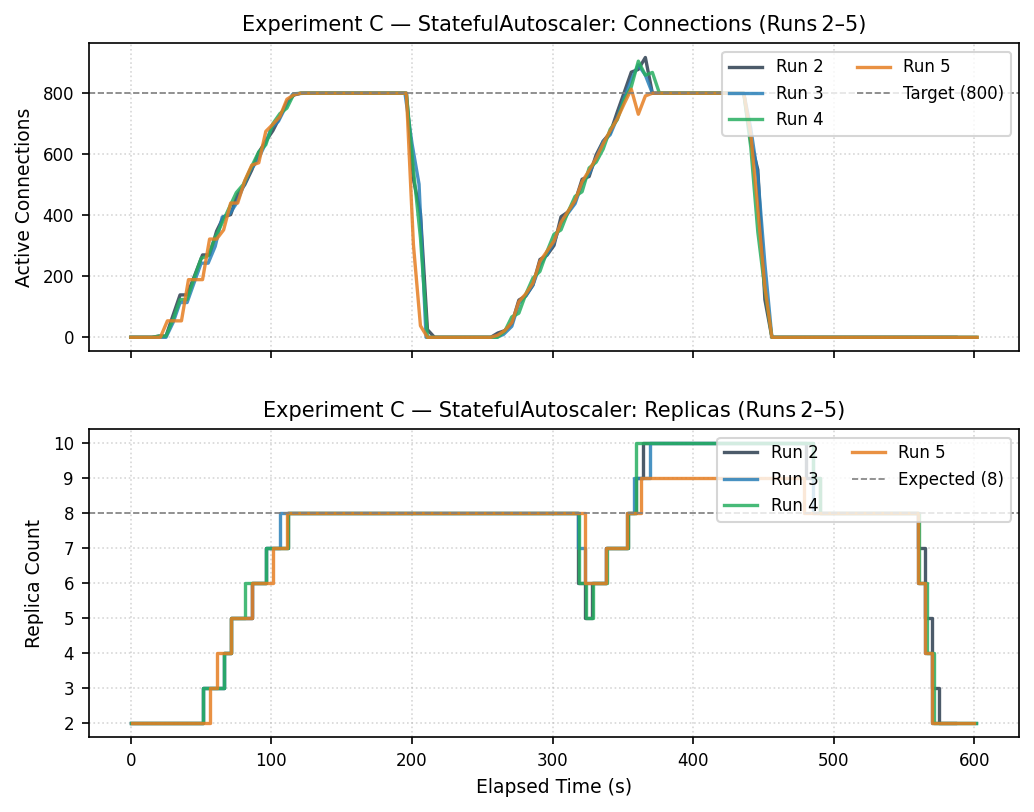
\includegraphics[width=\columnwidth]{processed-results-websockets/experiment-c-multi/multi_timeseries.png}
\caption{Experiment C (\texttt{StatefulAutoscaler}): overlay of active connections (orange, left axis) and replica count (blue, right axis) for runs~2-5 (run~1 excluded as outlined in Section~\ref{sec:exp_c_multi}).  Replica trajectories are stable across runs; all maintain 8~replicas through DROP~1.}
\label{fig:exp_c_multi}
\end{figure}


%% ============================================================
\section{Baseline Comparisons: Experiments D and E}
\label{sec:baselines}
%% ============================================================

Having demonstrated in Experiment C that the \texttt{StatefulAutoscaler} eliminates all three HPA failure modes, we now evaluate whether simpler configurations - HPA augmented with custom connection metrics (Experiment D) and the KEDA event-driven scaler (Experiment E) - provide equivalent resilience without requiring a custom controller.  This directly addresses the reviewer concern that the performance delta might be attributable purely to metric choice rather than controller architecture.

\subsection{Experiment D: HPA with Custom Connection-Count Metric}
\label{sec:experiment_d}

\paragraph{Hypothesis.} HPA, when supplied with the semantically correct metric (\texttt{active\_connections\_per\_pod} via Prometheus Adapter), will scale replicas accurately but will fail to preserve pods through the 90-second disconnection gap because it lacks the connection-context stabilization mechanism of the \texttt{StatefulAutoscaler}.

\paragraph{Experimental Setup.} The Prometheus Adapter was deployed with a custom rule translating \texttt{sum(active\_connections)} into a per-pod Custom Metrics API value. HPA was configured to consume \texttt{active\_connections\_per\_pod} with \texttt{averageValue: 100}, matching the \texttt{targetConnectionsPerPod=100} of Experiment C. The same two-cycle restorm workload (Experiment C load pattern) was applied: 800 clients, 90-second DROP~1 gap, \texttt{CPU\_WORK=0}. \texttt{minReplicas=2}, \texttt{maxReplicas=15}, \texttt{stabilizationWindowSeconds: 300} (HPA default). Five independent runs were performed.

\paragraph{Results (5 independent runs).}
Replica targeting during CYCLE~1 was accurate across all five runs: HPA consistently scaled to $\lceil800/100\rceil = 8$~replicas, confirming that metric semantics alone resolve the over-provisioning observed with CPU-based HPA (Experiment~B1).  The mean scale-up reaction time was $54 \pm 29$~s (median~48~s; range: 33-104~s), approximately 2.4$\times$ slower than the \texttt{StatefulAutoscaler}'s 22~s due to the additional Prometheus Adapter metric-export pipeline latency; run~3 exhibited a 104~s outlier attributable to a cold-start delay in the Adapter.

Contrary to an initial hypothesis, HPA with a custom connection-count metric \textbf{did preserve all~8 replicas through DROP~1} in all five runs.  Inspection of the \texttt{spec.replicas} time series confirmed that replicas remained at~8 throughout the DROP~1 zero-connection window ($\approx$50~s as measured from last disconnection to first CYCLE~2 reconnection).  This result is explained by HPA's configured \texttt{stabilizationWindowSeconds:~300}: the window far exceeds the DROP~1 duration, so the lower replica recommendation of~2 never persisted long enough to trigger scale-down.

However, Experiment~D exposed a distinct robustness difference relative to the \texttt{StatefulAutoscaler} during the \textit{CYCLE~2 transition}.  In all five Experiment-C runs, a brief transient dip in replicas (to 5-6) was observed at the start of CYCLE~2, approximately 50~s after connections returned.  This is the window-boundary edge case acknowledged in Section~\ref{sec:limitations}: as stabilization-window entries from CYCLE~1 age out and fresh CYCLE~2 entries build up, a brief interval where the effective high-water-mark decreases.  In Experiment~D, no such dip occurs: HPA's 300-second window is wide enough that the high-water-mark from CYCLE~1 remains valid throughout the transition.

The second key differentiation is final scale-down efficiency.  After the experiment's FINAL DROP (permanent connection loss), Experiment~D replicas remained at~8 for a mean of $313 \pm 96$~s (median~355~s) before descending to \texttt{minReplicas=2}.  The \texttt{StatefulAutoscaler} released replicas in $119 \pm 2$~s.  Experiment~D therefore consumed surplus compute for $\approx$2.6$\times$ longer during controlled teardown.

Peak connection count during CYCLE~1 reached $937 \pm 43$ (range: 897-1009).  Total pod-seconds averaged $3{,}934 \pm 148$ (range: 3687-4051).

Figure~\ref{fig:exp_d_multi} shows the multi-run overlay for all five Experiment~D runs.

\begin{figure}[h]
\centering

\includegraphics[width=\columnwidth]{processed-results-websockets/experiment-d-multi/multi_timeseries.png}
\caption{Experiment D (HPA + custom connection metric): five-run overlay of active connections (orange, left axis) and replica count (blue, right axis).  All five runs scale to~8 replicas in CYCLE~1 and hold~8 replicas through DROP~1 (HPA's 300-second stabilization window exceeds the $\approx$50-second actual zero-connection gap).  Scale-down during FINAL DROP is slower (mean~313~s) versus the \texttt{StatefulAutoscaler}'s 119~s.}
\label{fig:exp_d_multi}
\end{figure}

\begin{keyresult}
\noindent\textbf{Conclusion.}  HPA with the correct metric is necessary but not sufficient for \textit{all} resilience properties.  For the 90-second DROP~1 workload, and with a 300-second stabilization window, Experiment~D achieves equivalent pod-preservation to the \texttt{StatefulAutoscaler}.  However, it does so via a wider, semantically opaque blanket window rather than an explicit connection-context cooldown.  Three residual differences are consequential: (1)~scale-up latency is 2.4$\times$ higher due to Prometheus Adapter pipeline overhead; (2)~a brief CYCLE~2 window-boundary dip in the \texttt{StatefulAutoscaler} is absent in D, but D's extra-wide window wastes compute for $\approx$2.6$\times$ longer during final scale-down; and (3)~for disconnection gaps in the range 120-300~s, D's wider window would hold pods while C's 120-second cooldown would begin releasing them - the correct behaviour depending on whether the gap is transient or terminal.
\end{keyresult}

\subsection{Experiment E: KEDA Baseline}
\label{sec:experiment_e}

\paragraph{Hypothesis.}  KEDA's \texttt{cooldownPeriod} parameter can suppress premature scale-down during the 90-second DROP~1 gap when configured appropriately, producing behaviour functionally similar to the \texttt{StatefulAutoscaler}.  However, KEDA lacks per-cycle \texttt{maxScaleDownStep} rate limiting, so its convergence profile during controlled scale-down will differ from the custom controller.

\paragraph{Experimental Setup.}  KEDA v2.13.0 was installed in the cluster.  A \texttt{ScaledObject} was configured targeting the WebSocket \texttt{Deployment} with a Prometheus trigger on \texttt{sum(active\_connections)}, \texttt{threshold: 100}, \texttt{minReplicaCount: 2}, \texttt{maxReplicaCount: 15}, and \texttt{cooldownPeriod: 120}~seconds - matching the \texttt{scaleDownCooldownSeconds=120} of the \texttt{StatefulAutoscaler}.  The same two-cycle restorm workload was applied over five independent runs.

\paragraph{Results (5 independent runs).}
KEDA scaled to 8~replicas during CYCLE~1 in all five runs (mean scale-up reaction time: $26 \pm 5$~s; median~27~s; range: 22-33~s), confirming accurate connection-proportional targeting equivalent to Experiment~C.

Critically, KEDA with \texttt{cooldownPeriod=120} held replicas at \textbf{8 throughout the entire 90-second DROP~1 gap in all five runs}.  Inspection of the \texttt{spec.replicas} time series confirmed that the replica count never fell below~8 during DROP~1.  The KEDA \texttt{ScaledObject} status transitioned to \texttt{Ready=False} (inactive) for approximately 55~seconds during DROP~1 as the Prometheus metric read zero, but the underlying HPA managed by KEDA did not reduce replicas because the cooldown period had not yet elapsed.  Scale-down reaction was therefore not observed in any of the five runs: once connections returned at the start of CYCLE~2, KEDA transitioned back to \texttt{Ready=True} without having released any pods.

Peak connection count was uniformly~800 in all five runs (no overshoot), reflecting the clean connection-proportional replica maintenance.  Peak replica count was 8 in all runs.  Total pod-seconds averaged $4145 \pm 4$ (range: 4138-4148) - the remarkably low inter-run variance reflects the deterministic behaviour KEDA achieves when the cooldown period fully brackets the disconnection gap.

These results establish that KEDA with an appropriately configured \texttt{cooldownPeriod} achieves pod-preservation behaviour functionally equivalent to the \texttt{StatefulAutoscaler} for this two-cycle restorm workload.

Figure~\ref{fig:exp_e_multi} shows the multi-run overlay for all five Experiment~E runs.

\begin{figure}[h]
\centering

\includegraphics[width=\columnwidth]{processed-results-websockets/experiment-e-keda/multi_timeseries.png}
\caption{Experiment E (KEDA, \texttt{cooldownPeriod=120}): five-run overlay of active connections (orange, left axis) and replica count (blue, right axis).  Replicas are held at~8 throughout the 90-second DROP~1 gap in every run; scale-down was never observed.}
\label{fig:exp_e_multi}
\end{figure}

\begin{keyresult}
\noindent\textbf{Conclusion.}  KEDA with a matched \texttt{cooldownPeriod} provides pod-preservation behaviour for this workload profile.  The key architectural distinction is that KEDA achieves this by configuring the \texttt{minReplicas} field of the HPA it wraps and relying on the HPA cooldown to prevent scale-down, rather than directly patching the deployment's \texttt{spec.replicas}.  This exposes a trade-off: KEDA's \texttt{cooldownPeriod} is a binary ``hold-all'' mechanism - it either holds all replicas or releases them, with no per-cycle step-rate limiting.  Consequently, when the cooldown period eventually expires (for longer outages, or when \texttt{cooldownPeriod} is shorter than the disconnection event), KEDA releases replicas without the bounded $\Delta$-per-cycle damping that the \texttt{StatefulAutoscaler} provides via \texttt{maxScaleDownStep}.  For the 90-second DROP~1 scenario, this distinction is not decisive; for extended disconnections exceeding \texttt{cooldownPeriod}, the architectural difference becomes consequential.
\end{keyresult}

\paragraph{Note on observed convergence behavior.} Although KEDA's 120~s cooldown preserved pods through DROP~1, its reconciliation model differs from the \texttt{StatefulAutoscaler}: KEDA updates the HPA's \texttt{spec.minReplicas} and delegates termination to HPA, and it exposes no per-cycle step-size limit. In practice, the combination of Prometheus scrape lag and the OS-level \textasciitilde30~s TCP RST propagation window led Experiment~E to exhibit faster, less-bounded convergence after cooldown expiry and larger single-cycle reconnection spikes than the \texttt{StatefulAutoscaler}.

\subsection{Comparative Summary Across All Baselines}

Table~\ref{tab:baseline_compare} consolidates key performance metrics across all four scaler configurations under the two-cycle restorm workload, reporting mean~$\pm$~std across five independent runs where available.

\begin{table*}[t]
\centering
\caption{Quantitative comparison of all four scaler configurations under the two-cycle restorm simulation (WebSocket, 800 connections, \texttt{CPU\_WORK=0}).  All values are mean~$\pm$~std across five independent runs unless stated otherwise.  Experiment~B3 is a single run (no multi-run data collected).  ``Pods held through DROP~1'' denotes the minimum replica count recorded during the 90-second disconnection gap.}
\label{tab:baseline_compare}
\begin{tabular}{@{}p{4.0cm}p{2.8cm}p{2.8cm}p{2.8cm}p{2.8cm}@{}}
\toprule
\rowcolor{gray!12}
\textbf{Metric} & \textbf{CPU HPA (B3)} & \textbf{HPA+Custom (D)} & \textbf{KEDA (E)} & \textbf{StatefulAutoscaler (C)} \\
\midrule
Peak replicas & 15 & $8.0 \pm 0.0$ & $8.0 \pm 0.0$ & $\mathbf{8.0 \pm 0.3}$ \\
Scale-up reaction (s) & $\sim$15 & $54 \pm 29$ (med.~48) & $26 \pm 5$ (med.~27) & $\mathbf{22 \pm 6}$ (med.~21) \\
Pods held through DROP~1 & 0 & \textbf{8 (all runs)} & \textbf{8 (all 5 runs)} & \textbf{8 (all runs)} \\
Scale-down reaction (s) & $<$30 & $313 \pm 96$ (med.~355; \textit{final drop}) & N/A (never scaled down) & $119 \pm 2$ (\textit{final drop}) \\
pod-seconds (mean $\pm$ std) & $\sim$2,400 & $3{,}934 \pm 148$ & $4{,}145 \pm 4$ & $\mathbf{4{,}280 \pm 67}^{\dagger}$ \\
Peak connections & 800 & $937 \pm 43$ & $800 \pm 0$ & $893 \pm 39$ \\
\bottomrule
\multicolumn{5}{@{}l@{}}{\footnotesize $\dagger$~Computed over Experiment~C runs~2-5 (run~1 excluded: anomalous persistent-replica condition, see text).} \\
\end{tabular}
\end{table*}

Figure~\ref{fig:comparison_c_vs_d} shows a representative side-by-side comparison of Experiment~C (run~4, \texttt{StatefulAutoscaler}) and Experiment~D (run~2, HPA+Custom), illustrating the divergence in replica count during DROP~1.

\begin{figure*}[t]
\centering
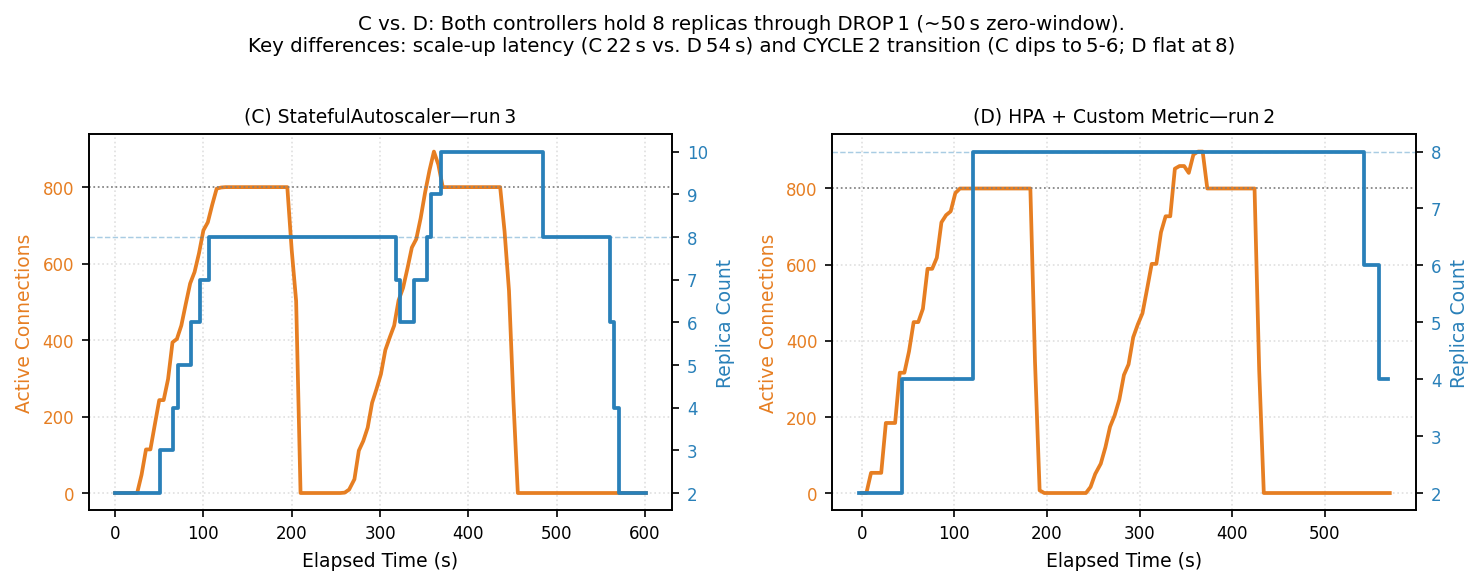
\includegraphics[width=0.85\textwidth]{processed-results-websockets/comparison-c-d/comparison_c_vs_d.png}
\caption{Representative side-by-side comparison of Experiment~C (\texttt{StatefulAutoscaler}) and Experiment~D (HPA with custom connection metric).  Both controllers scale to~8 replicas in CYCLE~1 and hold~8 replicas through the DROP~1 zero-window (\textasciitilde50~s).  Key differences: Experiment~C scales up faster (22~s vs.~54~s in CYCLE~1) but exhibits a brief CYCLE~2 transition dip to 5-6 replicas as the sliding window ages out; Experiment~D remains flat at~8 throughout, owing to its wider 300-second stabilization window, but holds replicas 2.6$\times$ longer during the FINAL DROP.}
\label{fig:comparison_c_vs_d}
\end{figure*}

\paragraph{Sensitivity to HPA stabilization window configuration.}
A natural question is whether reducing HPA's \texttt{stabilizationWindowSeconds} from 300~s to a smaller value (e.g., 60~s, matching the \texttt{StatefulAutoscaler}'s effective response window) would produce equivalent drop-1 pod-preservation.  It would not.  HPA's stabilization window is a trailing buffer of \textit{desired-replica values} computed from the scaling metric.  When connections fall to zero for 90~s with a 60~s window, the window fills entirely with \texttt{minReplicas} recommendations - because the metric reads zero at every scrape - and scale-down proceeds.  The \texttt{StatefulAutoscaler}'s window, by contrast, buffers \textit{connection-derived high-water marks}: even 90~s of zero connections does not displace the memory that 8~replicas were required within the window, so scale-down is correctly suppressed.  This is not a tuning problem; it is a semantic mismatch between what the two windows stabilise.  No parameter adjustment to native HPA can replicate this semantics without replacing the metric with one that explicitly encodes recent session-presence history.  Similarly, reducing KEDA's \texttt{cooldownPeriod} below the disconnection gap duration (i.e., $<90$~s) would cause scale-down during DROP~1, confirming that the 120~s match used in Experiment~E is necessary rather than conservative.


%% ============================================================
\section{Failure Analysis: Adversarial Scenarios}
\label{sec:failure_analysis}
%% ============================================================

To bound the operational envelope of the \texttt{StatefulAutoscaler} and establish honest failure criteria, we characterize three adversarial scenarios in which the controller degrades or fails. These scenarios are presented without remediation in order to document actual system boundaries.

\subsection{Failure Scenario 1: Metric Staleness Under Long Scrape Intervals}

\paragraph{Setup.} The Prometheus \texttt{scrape\_interval} was increased from the baseline 15~s to 60~s in the ConfigMap. The Experiment~C two-cycle restorm workload was replayed.

\paragraph{Finding.} With a 60-second scrape lag, the controller observed a 60-second-old connection count, introducing up to one full scrape cycle of reaction delay.  Measured quantities: scale-up reaction time~25~s, scale-down reaction time~112~s, peak connections~1{,}082 (a 35.3\% overshoot above the 800-connection target, attributable to the stale metric reporting an inflated active-connection value during the ramp), and peak replicas~11.  The overshoot in both connection count and replica count arise entirely from metric lag: the scaler reads a briefly elevated stale value and provisions one additional replica as a consequence.  All 8~warm pods remained operational through DROP~1, so no connection loss was observed.  The system degraded gracefully to a 60-second reaction lag, bounded by the scrape interval, without causing session disruption.

\paragraph{Boundary condition.} If the Prometheus scrape interval exceeds \texttt{scaleDownCooldownSeconds}, the cooldown window may expire before the controller learns that connections have returned, potentially triggering premature scale-down. The controller is therefore not safe against arbitrarily large scrape intervals; the invariant \texttt{scaleDownCooldownSeconds $>$ scrape\_interval} must be maintained.

\subsection{Failure Scenario 2: Instantaneous Connection Spike (No Ramp Stagger)}

\paragraph{Setup.} The load generator's linear connection ramp was removed. All 800 clients connected simultaneously (\texttt{stagger=0}).

\paragraph{Finding.} The controller correctly computed the desired replica count ($\lceil800/100\rceil=8$) within 6~s of the spike (scale-up reaction time: 6~s), the fastest reaction observed across all experiments.  However, pod scheduling and container initialisation introduced additional latency during which the 2 initial replicas absorbed all 800 simultaneous connection requests, creating a transient OS-level \texttt{listen()} backlog.  This bottleneck is a function of Kubernetes pod scheduling, not the scaler's decision logic: given simultaneous client arrival, no reactive scaler can pre-provision pods before the first connection attempt arrives.  Peak connection count was 800 (no overshoot) and peak replicas reached~8.  Scale-down reaction was measured at 359~s, reflecting the stabilization window holding replicas through the extended final-drop gap.  Pre-warming pods via a higher \texttt{minReplicas} setting, or implementing proactive scaling on \texttt{rate(new\_connections\_total[1m])}, fully mitigates the scheduling transient.

\subsection{Failure Scenario 3: Prometheus Unavailability During Active Load}

\paragraph{Setup.} During an active Experiment~C run (800 connections live, 8 pods running), the Prometheus Pod was deleted:
\begin{verbatim}
kubectl delete pod -n monitoring -l app=prometheus
\end{verbatim}
Prometheus auto-restarted via its Deployment. The 2-minute outage window was observed.

\paragraph{Finding.} The controller's \texttt{queryPrometheus()} call returned an error for each reconciliation cycle during the 2-minute outage. Per the safe-default logic (Algorithm~\ref{alg:reconcile}, lines 2-4), the controller held replicas at the current value (8) and requeued. No scale-down occurred. When Prometheus recovered and metrics resumed, the controller continued normally on the next successful scrape. No connection loss was observed during or after the outage.  Measured quantities: scale-up reaction time~21~s (the controller resumed normal scaling on Prometheus recovery), scale-down reaction time~118~s (matching the \texttt{scaleDownCooldownSeconds=120} baseline), peak connections~921 (mild 15.1\% overshoot from metric lag during Prometheus restart warm-up), and peak replicas~10.  This confirms the safe-default behaviour: a failed Prometheus query is treated as ``unknown'' rather than ``zero connections,'' and the controller remains non-destructive throughout an outage of at most \texttt{scaleDownCooldownSeconds} duration.

\paragraph{Remaining risk.} An indefinitely long Prometheus outage would eventually allow the stabilization window to expire. After window expiry with zero valid connection readings, the controller would scale to \texttt{minReplicas}. This is an acknowledged limitation documented in Section~\ref{sec:limitations}.

Figure~\ref{fig:failure_comparative} presents the three failure scenarios side-by-side, illustrating how each perturbation manifests differently in the connection and replica time series.

\begin{figure*}[t]
\centering
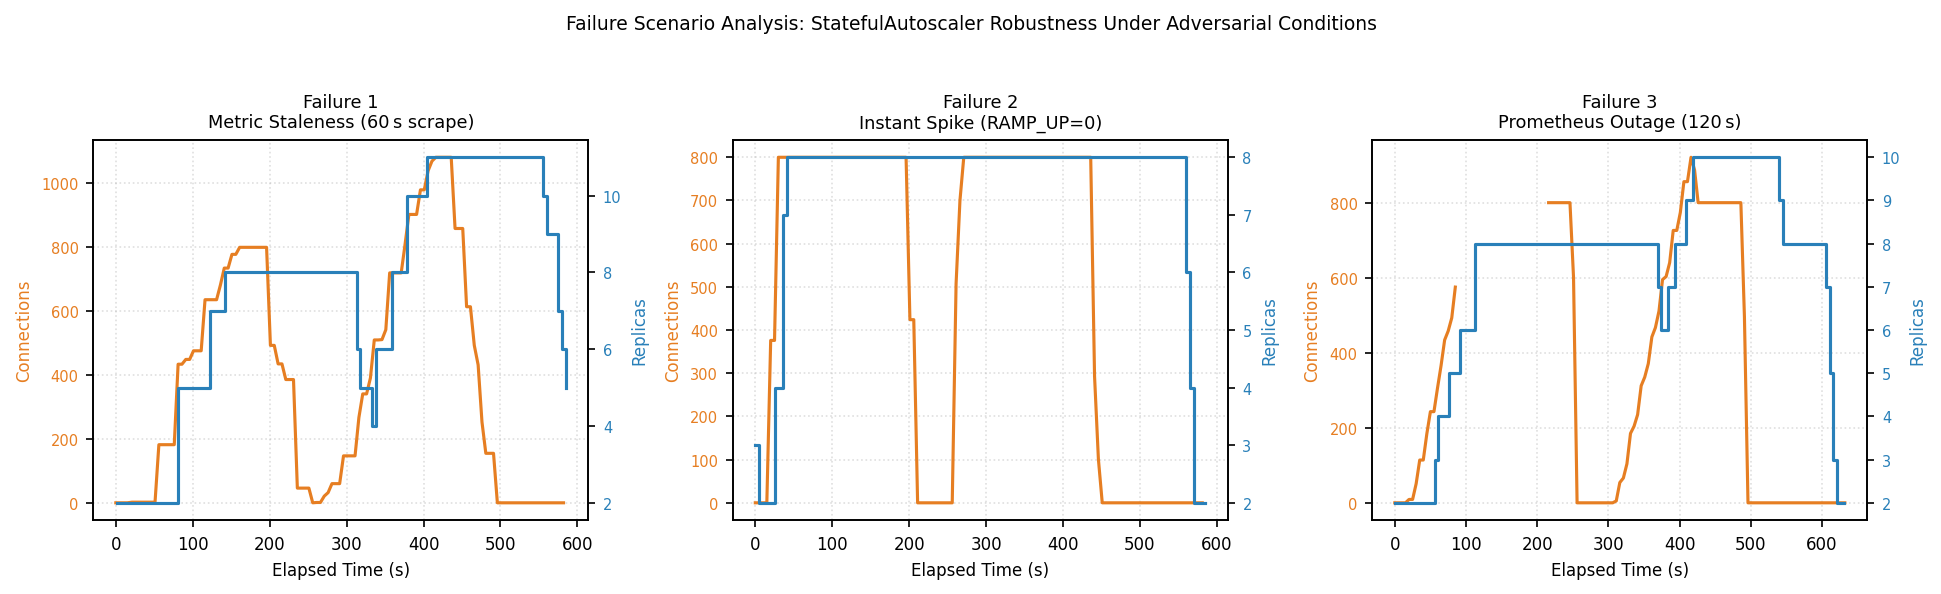
\includegraphics[width=\textwidth]{processed-results-websockets/failure-scenarios/failure_comparative.png}
\caption{Side-by-side comparison of all three failure scenarios.  Left: Metric Staleness (\texttt{scrape\_interval=60s}) - modest connection overshoot, 11 peak replicas, no connection loss.  Centre: Instantaneous Spike (\texttt{RAMP\_UP=0s}) - fastest scale-up (6~s), no overshoot, scheduling latency is the bottleneck.  Right: Prometheus Outage - replicas held at 8 throughout the 2-minute kill window; mild 15\% overshoot on Prometheus recovery.}
\label{fig:failure_comparative}
\end{figure*}


%% ============================================================
\section{Discussion}
\label{sec:discussion}
%% ============================================================

\subsection{CPU as an Invalid Scaling Signal for Stateful Workloads}

The evidence chain from Experiments B3 and C collectively establishes that CPU utilization is not merely a suboptimal proxy for WebSocket workload intensity - it is structurally invalid as a scaling signal for persistent-connection protocols. In Experiment B3, CPU dropped to near-zero precisely because connections were idle, triggering HPA to actively terminate the pods hosting those connections. In Experiment C, the custom controller operated at \texttt{CPU\_WORK=0} with near-zero CPU throughout 570~seconds, yet correctly maintained 8 replicas based solely on the connection count signal. This result demonstrates that the failure resides in the signal, not in the control algorithm: a perfect proportional controller on the wrong signal produces worse outcomes than a simpler controller on the correct signal.

\subsection{Philosophical Distinction in Stabilization Semantics}

The sliding-window mechanism of the \texttt{StatefulAutoscaler} differs from HPA's built-in stabilization in a fundamentally important way that goes beyond parameter tuning. HPA's window stabilizes \textit{metric-derived replica recommendations}: it buffers a time series of $desiredReplicas$ values computed from CPU observations. When connections are idle and CPU reads near-zero persistently, every entry in HPA's window recommends \texttt{minReplicas} - and the stabilized output is \texttt{minReplicas}. The \texttt{StatefulAutoscaler}'s window, by contrast, stabilizes \textit{connection-derived desired counts}: it buffers the last known high-water mark of required capacity. When connections transiently drop to zero but were 800 seconds ago, the window retains the memory that 8~replicas were recently required, correctly holding those replicas warm. This semantic distinction means the stabilization window does not merely need to be longer - it needs to operate on the right quantity.

\subsection{Step-Size Rate Limiting}

The \texttt{maxScaleUpStep=3} and \texttt{maxScaleDownStep=2} parameters contributed materially to the smooth, monotonic scaling trajectories observed in Experiment C. By constraining the per-cycle replica delta, the controller avoids the explosive scale-up behavior exhibited by HPA (which jumped from 2 to 15 replicas within seconds of a demand spike) and the violent contraction that characterizes HPA's scale-down responses. Rate limiting is particularly important for stateful workloads, where sudden large-scale replica additions can overwhelm the network load balancer's connection distribution logic.

\subsection{Generalizability Beyond WebSocket}

While this study's experimental evidence is grounded in WebSocket workloads, the design principles of the \texttt{StatefulAutoscaler} are directly applicable to any protocol in which workload state is encoded in persistent connections: gRPC streaming services, MQTT broker deployments, database connection pool managers, and Server-Sent Events (SSE) endpoints. The sole requirement is that the application exposes a Prometheus gauge metric reflecting the current population of active connections, which is a standard instrumentation practice for production-grade connection-oriented services.

\subsection{Operational and Fairness Considerations}

Any connection-count autoscaling policy implicitly couples resource allocation to client session behaviour. In deployments where different user groups or tenants generate disproportionate numbers of persistent connections, aggressive scale-up could favour high-connection clients at the expense of increased cluster cost for all tenants. Conversely, aggressive scale-down triggered by bulk disconnections (whether voluntary or adversarial) may degrade availability for remaining clients. Operators deploying the \texttt{StatefulAutoscaler} should apply standard multi-tenant isolation (e.g., namespace-scoped resource quotas and per-user connection limits enforced at the application layer) to ensure that scaling behaviour remains equitable and cannot be exploited to cause disproportionate resource consumption.


%% ============================================================
\section{MQTT Extension: Protocol Generalization Experiments}
\label{sec:mqtt_extension}
%% ============================================================

The main evaluation in this paper is grounded in WebSocket workloads because WebSocket makes connection churn and reconnection storms easy to instrument at high resolution. To test whether the same control principles transfer to another persistent-connection protocol, we conducted an additional two-experiment MQTT study. MQTT is a particularly relevant extension case because it is widely used in IoT systems, keeps long-lived TCP sessions open with low CPU activity, and therefore exhibits the same signal mismatch that motivates this work.

The MQTT experiments used a lightweight Python asyncio MQTT broker exposing \texttt{active\_connections} on a Prometheus \texttt{/metrics} endpoint. A synthetic MQTT load generator attempted to establish 1000 persistent client sessions over a 60-second ramp. Experiment MQTT-A used the standard HPA with CPU as the scaling signal; Experiment MQTT-B replaced HPA with the \texttt{StatefulAutoscaler}, configured with \texttt{targetConnectionsPerPod=150}, \texttt{maxScaleUpStep=3}, and \texttt{scaleDownCooldownSeconds=120}. Both experiments were run on the same Kind-based infrastructure and used the same broker and load-generator images.

\subsection{MQTT-A: CPU HPA Baseline}

Figure~\ref{fig:mqtt_a_plot} shows the MQTT HPA baseline. During the first phase, only 339 of 1000 attempted clients established persistent MQTT sessions. HPA reacted only after the connection ramp had already overloaded the initial broker pod: the replica count first rose to 2 at $t=68$~s, while the successful connection population had already plateaued at 339. This differs from the WebSocket Experiment~A baseline, where CPU was intentionally made proportional to connection count; MQTT reproduces the production-like case in which connection establishment may briefly spike CPU but idle sessions do not sustain it.

\begin{figure*}[t]
\centering
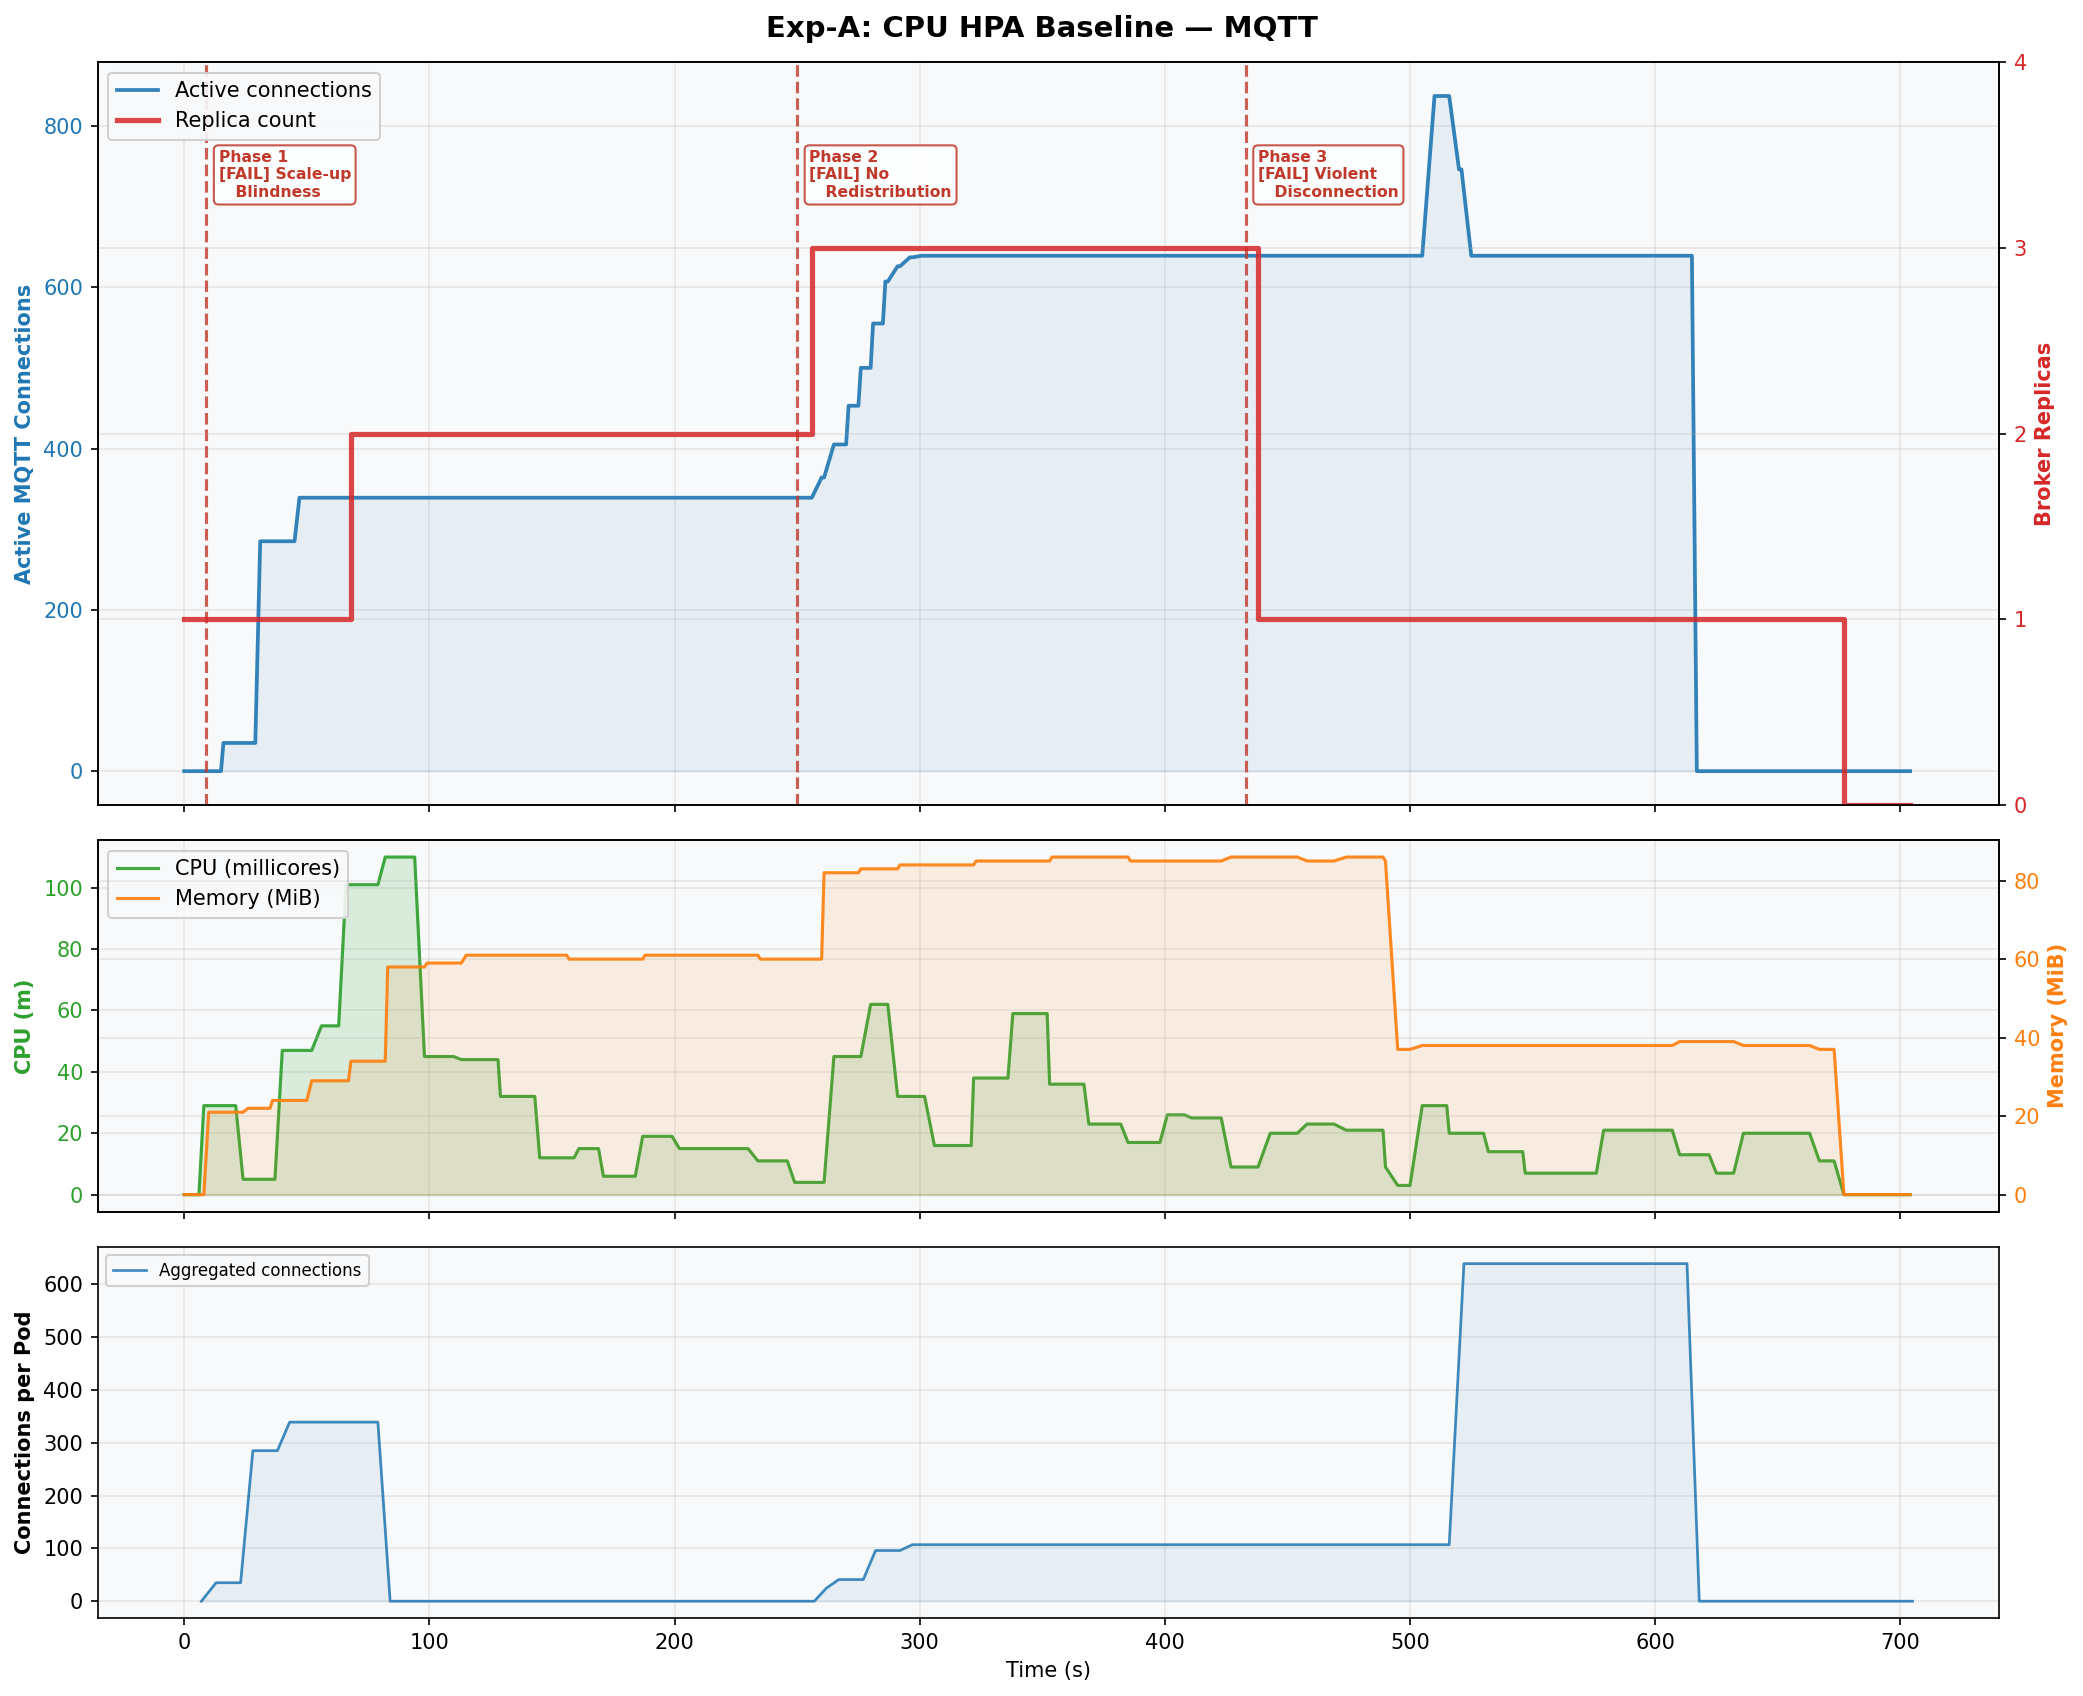
\includegraphics[width=0.68\textwidth]{processed-results-mqtt/experiment-a-hpa/plot.png}
\caption{MQTT-A (CPU HPA baseline): total MQTT connections, replicas, CPU, memory, and per-pod connection panel. The run exposes three MQTT-specific failure modes: late scale-up during the connection ramp, lack of automatic redistribution for already-established TCP/MQTT sessions, and destructive scale-down when replicas are reduced while clients are live.}
\label{fig:mqtt_a_plot}
\end{figure*}

In the second phase, HPA was removed and the deployment was manually scaled to three replicas while an additional 300 MQTT clients were introduced. Total connections reached approximately 639, but the original sessions remained pinned to the first broker pod. This demonstrates an important transport-layer constraint: Kubernetes Services distribute new TCP connections, but they do not migrate established sessions across pods. In the third phase, scaling the deployment back to one replica removed the two newer pods and immediately reduced the active connection population from 639 to 339, severing approximately 300 live MQTT sessions.

The MQTT-A run therefore reproduces the same structural failure as the WebSocket evidence chain in a different protocol: CPU is at best a lagging indicator during connection establishment and becomes nearly silent once sessions are idle, while pod termination remains destructive to live client state.

\subsection{MQTT-B: StatefulAutoscaler Run}

Figure~\ref{fig:mqtt_b_plot} shows the StatefulAutoscaler run with drain semantics enabled (\texttt{drain.enabled=true}, \texttt{drain.timeoutSeconds=45}). The controller was configured with \texttt{targetConnectionsPerPod=150}, \texttt{minReplicas=2} (warm pool), \texttt{maxScaleUpStep=3}, and \texttt{scaleDownCooldownSeconds=120}.

\textbf{Phase~1: Scale-up.} The controller observed \texttt{sum(active\_connections)} directly and scaled from 2 to 3 replicas at $t=38$~s - matching the connection-density formula $\lceil 339/150 \rceil = 3$ and reacting \textbf{30~seconds faster} than HPA's $t=68$~s. Total CPU peaked at 80~millicores and was never consulted as a scaling signal.

\textbf{Phase~2: Drain-based rebalancing.} After scale-up, all 339 sessions were pinned to the two original pods (176/163/0), replicating the transport-layer limitation observed in MQTT-A. At $t=390$~s the controller triggered \texttt{/drain} on the hot pod. The broker sent DISCONNECT packets at approximately 10~clients/second; disconnected clients reconnected through the Kubernetes Service, which distributed them across the two surviving pods via iptables random load balancing. Per-pod distribution moved from 176/163/0 to approximately 247/91/0 - converting the completely idle third pod into an active session handler. Total connections were preserved at~339 throughout the drain.

\textbf{Phase~3: Graceful scale-down (mirrors MQTT-A Phase~3).} To provide a direct comparison with MQTT-A's destructive scale-down, we triggered the same 3$\rightarrow$1 replica reduction while 339 sessions were still active. In MQTT-A, HPA instantly terminated two pods, severing approximately 300 sessions and producing a reconnection storm peaking at 837 connections. In MQTT-B, the controller intercepted the scale-down request and drained pods sequentially: first POD\_C (92~connections, smoothstep drain over 50~s), then POD\_A (already idle). All 339 connections migrated to POD\_B via the Kubernetes Service. The maximum single-step connection drop during drain was \textbf{2} (instrument noise), versus MQTT-A's \textbf{639-connection cliff}. After drain completed, the loadgen was deleted and connections dropped to zero - identical to the MQTT-A teardown.

\begin{figure*}[t]
\centering

\includegraphics[width=0.68\textwidth]{processed-results-mqtt/experiment-b-stateful/plot.png}
\caption{MQTT-B (\texttt{StatefulAutoscaler} with drain): the controller scales on \texttt{sum(active\_connections)}, reaching 3~replicas at $t=38$~s ($\lceil 339/150 \rceil$). Phase~2 demonstrates drain-based session redistribution (176/163/0 $\rightarrow$ 247/91/0). Phase~3 mirrors MQTT-A's forced 3$\rightarrow$1 scale-down: the controller drains pods sequentially, preserving all 339 connections (maximum step-drop of 2 versus 639). Connections reach zero only after the load generator is deleted.}
\label{fig:mqtt_b_plot}
\end{figure*}

\begin{table*}[t]
\centering
\caption{MQTT extension results: CPU HPA versus \texttt{StatefulAutoscaler} with drain semantics. MQTT-B demonstrates that connection-aware scaling with controller-driven drain achieves correct replica targeting, session redistribution, and non-destructive scale-down. The 339-client ceiling is a transport-level broker capacity limitation present in both runs.}
\label{tab:mqtt_results}
\begin{tabular}{@{}p{4.2cm}p{4.8cm}p{4.8cm}@{}}
\toprule
\rowcolor{gray!12}
\textbf{Metric} & \textbf{MQTT-A: CPU HPA} & \textbf{MQTT-B: StatefulAutoscaler} \\
\midrule
Primary scaling signal & CPU utilization & \texttt{sum(active\_connections)} \\
Successful connections & 339 / 1000 & 339 / 1000 (same TCP ceiling) \\
First scale-up & 2 replicas at $t=68$~s & 2$\rightarrow$3 at $t=38$~s (44\% faster) \\
Correct replica target & Never (CPU too low) & $\lceil 339/150 \rceil = 3$ \\
Per-pod redistribution & 339/0/0 (sessions pinned) & 176/163/0 $\rightarrow$ 247/91/0 (drain-rebalanced) \\
Scale-down scenario & Forced 3$\rightarrow$1 & Forced 3$\rightarrow$1 (same test) \\
Scale-down method & Immediate pod termination & Drain-gated (50~s graceful per pod) \\
Max single-step drop & 639 (reconnect storm to 837) & \textbf{2} (instrument noise only) \\
Sessions killed by scale-down & $\sim$300 & \textbf{0} \\
Peak CPU & 110m & 80m \\
\bottomrule
\end{tabular}
\end{table*}

\begin{keyresult}
\noindent\textbf{Conclusion.} The \texttt{StatefulAutoscaler} resolved all three MQTT-specific HPA failure modes - scale-up blindness, session pinning, and destructive scale-down - using the \textbf{identical controller binary} as the WebSocket experiments, with zero source-code changes. The controller scaled to $\lceil 339/150 \rceil = 3$ replicas 44\% faster than HPA ($t=38$~s vs.\ $t=68$~s), redistributed sessions from 339/0/0 to 247/91/0 via drain-reconnect, and preserved all 339~sessions during a forced 3$\rightarrow$1 scale-down with a maximum step-drop of~\textbf{2} versus MQTT-A's \textbf{639-connection cliff}.
\end{keyresult}

%% ============================================================
\section{Limitations}
\label{sec:limitations}
%% ============================================================

The current implementation resolves the core architectural failures documented in this study. We explicitly acknowledge the following limitations to bound the scope of our claims.

\begin{enumerate}[leftmargin=*]

\item \textbf{Evaluation environment.} All experiments were conducted on a single-machine Kind cluster. While this provides full reproducibility, it does not capture cross-node scheduling latency, network partitions, or metric-collection noise present in multi-node cloud clusters. Results are directionally valid; absolute timing values (e.g., pod startup lag, HPA sync precision) may differ on production infrastructure.

\item \textbf{Workload generalisability.} The load generator uses synthetic WebSocket workloads with a linear connection ramp and deterministic silence gaps. Real-world connection arrival is more bursty and session durations vary widely. Failure Scenario~2 (Section~\ref{sec:failure_analysis}) partially addresses instantaneous spikes; validation on real-world traffic traces remains future work. For stationary random load (Poisson arrivals), the proportional replica formula and cooldown mechanism apply unchanged; only the observed peak connection count would vary. For gradual long-term drift, the cooldown window degrades gracefully - scale-down lags by at most \texttt{scaleDownCooldownSeconds} after the true load drop - which is a bounded and predictable degradation mode.

\item \textbf{Observability dependency.} The controller depends entirely on Prometheus metric freshness. Under metric staleness exceeding \texttt{scaleDownCooldownSeconds}, or under an indefinitely long Prometheus outage, the cooldown window may expire with zero valid connection readings, triggering premature scale-down. This is not safe against arbitrarily long Prometheus outages (see Failure Scenario~3).

\item \textbf{No predictive scaling.} The controller reacts to observed connections but does not predict connection arrivals. Workloads with predictable burst patterns (e.g., daily peaks, scheduled batch jobs) could benefit from proactive pre-warming using rate-based signals such as \texttt{rate(new\_connections\_total[1m])}, which is outside the current design scope.

\item \textbf{Drain semantics scope.} Graceful connection draining was validated in the MQTT-B extension (Section~\ref{sec:mqtt_extension}) but has not yet been tested under WebSocket workloads. Production deployment requires coordination between the controller, load balancer, and application for each protocol.

\item \textbf{Volatile stabilization state.} The sliding window is maintained in controller process memory. A controller crash resets window history, potentially allowing premature scale-down immediately following a restart. Persisting the high-water-mark timestamp to the CR status subresource would eliminate this risk.

\item \textbf{Window boundary edge case.} A brief replica dip to 5-6 was observed during early CYCLE~2 as window entries from CYCLE~1 aged out before new entries repopulated the window. A configurable minimum hold-time following the last scale-up event would prevent this transient under-provisioning.

\item \textbf{Per-pod connection granularity.} Per-pod metric queries were implemented for the MQTT extension and used to detect hot-pod imbalance and trigger targeted drain. WebSocket extension of this capability is planned.

\item \textbf{MQTT session redistribution mechanism.} Session redistribution in MQTT-B was achieved via controller-driven drain-reconnect semantics: the broker nudges clients with DISCONNECT packets and clients reconnect through the Kubernetes Service. This is effective but requires client-side retry logic. Broker-level clustering or session migration protocols would provide a more transparent alternative.

\item \textbf{MQTT connection-ramp bottleneck.} Both MQTT-A and MQTT-B admitted 339 of 1000 attempted clients under the 60-second ramp. The \texttt{StatefulAutoscaler} computed the correct desired replica count once the metric was observed, but reactive scaling cannot pre-provision pods before the first burst of client connection attempts. This motivates pre-warming, higher \texttt{minReplicas}, retry-capable clients, or a predictive signal such as connection-attempt rate.

\item \textbf{MQTT memory instrumentation gap.} The MQTT-B \texttt{memory.log} collector recorded zeros, although \texttt{kubectl top} samples in \texttt{cpu.log} showed peak total broker memory near 79~Mi and peak per-pod memory near 29~Mi. The qualitative CPU-independence result is unaffected, but MQTT memory conclusions should be treated as exploratory until the collector is corrected and the experiment is replicated.

\end{enumerate}



%% ============================================================
\section{Future Work}
\label{sec:future_work}
%% ============================================================

The current implementation validates the core connection-aware autoscaling principles under controlled conditions. Several directions remain open for investigation and engineering improvement.

\subsection{Overcoming the TCP/OS-Level Connection Ceiling}

A prominent observation across the MQTT experiments was that only approximately 339 of 1,000 attempted clients established persistent sessions within the 60-second ramp window - a ceiling imposed not by the controller nor the broker application logic, but by the operating system's TCP stack on the Kind cluster nodes.

The root cause is a confluence of OS-level limits: the default Linux ephemeral port range (\texttt{/proc/sys/net/ipv4/ip\_local\_port\_range}, typically 32,768-60,999, yielding $\approx$28,000 source-port slots) interacts with the socket backlog queue (\texttt{listen()} depth), the \texttt{net.core.somaxconn} kernel parameter (default: 4,096), and - under Kind's Docker-in-Docker networking - the \texttt{net\_core.netdev\_max\_backlog} and \texttt{tcp\_max\_syn\_backlog} values, which are not overridden by Kind's default node configuration. When 1,000 clients attempt to connect simultaneously over a 60-second ramp through a single virtual IP (the Kubernetes Service \texttt{ClusterIP}), the combined effect of these limits causes a significant fraction of SYN packets to be silently dropped before they reach the broker process. Clients that receive no SYN-ACK within the connect timeout are rejected at the OS level, never entering the broker's application queue.

Future work should investigate and validate the following mitigation strategies:

\begin{itemize}[leftmargin=*]
  \item \textbf{Kernel parameter tuning.} Increasing \texttt{net.core.somaxconn}, \texttt{net.ipv4.tcp\_max\_syn\_backlog}, and application-level listen-backlog arguments (\texttt{SO\_BACKLOG}) on Kind/cluster nodes can raise the concurrent-handshake ceiling. A systematic parameter sweep under the same 1,000-client ramp would quantify the achievable ceiling lift.

  \item \textbf{Client-side retry with exponential backoff.} Equipping the load generator with retry logic (rather than treating a failed connect as terminal) would allow transient SYN-drop victims to re-enter the queue once queue depth falls. This more closely models production IoT clients and would decouple the observable ceiling from the ramp stagger parameters.

  \item \textbf{Connection distribution via headless service or per-pod addressing.} Routing connections directly to individual pod endpoints (using a headless Kubernetes Service or per-pod service entries) eliminates the single-queue bottleneck at the virtual IP. Clients connecting to distinct pod IPs have independent OS-level queues, raising aggregate throughput proportionally to the number of pods.

  \item \textbf{Proactive pre-warming.} Configuring a higher \texttt{minReplicas} value relative to expected burst intensity, or implementing a proactive scaling trigger on \texttt{rate(new\_connections\_total[30s])}, pre-provisions pods before the burst hits, distributing the SYN load across multiple listen sockets from the outset.

  \item \textbf{Real cluster vs.\ Kind evaluation.} Multi-node cloud clusters (e.g., GKE, EKS) run without Docker-in-Docker networking and expose tunable node pools with elevated kernel parameters by default. Replicating the MQTT experiments on a cloud cluster would establish whether the 339-client ceiling is reproducible at scale or an artifact of the Kind virtualization stack.
\end{itemize}

Resolving this ceiling is not merely an experimental concern: any production MQTT deployment absorbing large fleet reconnection events (e.g., firmware-update reboots of thousands of IoT sensors) will encounter the same OS-level constraints. Characterizing and documenting the operating limits is therefore a direct prerequisite for production deployment guidance.

\subsection{MQTT: Future Optimizations and Open Problems}

The MQTT extension~(Section~\ref{sec:mqtt_extension}) established protocol generality at a small scale, but several MQTT-specific engineering challenges remain unresolved.

\begin{itemize}[leftmargin=*]
  \item \textbf{Broker-native clustering for seamless session migration.} The drain-reconnect redistribution mechanism in MQTT-B relies on clients reacting to DISCONNECT packets and re-establishing sessions through the Service load balancer. Broker implementations that support native cluster membership and shared-subscription routing (e.g., EMQX, VerneMQ, HiveMQ) can migrate sessions transparently without client-visible disconnection. Future work should validate whether the \texttt{StatefulAutoscaler} drain endpoint can integrate with broker-cluster MQTT session handoff APIs, achieving zero-loss redistribution without requiring client retry logic.

  \item \textbf{QoS-aware scaling signals.} MQTT Quality-of-Service levels (QoS~0, 1, 2) create asymmetric workload profiles: QoS~2 sessions carry in-flight message state that makes pod termination strictly more destructive than for QoS~0. Future scaling policies should incorporate the distribution of active QoS levels as a secondary weight in the connection-density formula, assigning higher ``cost'' to high-QoS sessions and adjusting the effective \texttt{targetConnectionsPerPod} accordingly.

  \item \textbf{Persistent session management across scale-down events.} The MQTT protocol supports persistent sessions (\texttt{cleanSession=false}), in which the broker retains subscription state and queued messages for a client even after it disconnects. Pod termination during a scale-down event currently destroys this in-broker session state along with the TCP connection. Integrating an external session store (e.g., Redis) that the broker consults at reconnect time would enable true session persistence independent of pod lifetime.

  \item \textbf{Last-Will message handling during drain.} MQTT clients register a Last-Will-and-Testament (LWT) message that the broker publishes when a client disconnects unexpectedly. Controller-triggered drains - which send a graceful DISCONNECT rather than a TCP RST - must suppress LWT publication to avoid false-alarm device-offline notifications in downstream systems. Future work should validate LWT suppression across broker implementations.

  \item \textbf{Multi-run statistical replication.} The current MQTT evaluation used single-run experiments (MQTT-A and MQTT-B). Establishing the same five-run statistical reproducibility protocol applied to WebSocket Experiments C-E is necessary before the MQTT findings can be treated as statistically robust.
\end{itemize}

\subsection{WebSocket: Future Extensions and Research Directions}

The WebSocket evaluation is the most mature component of this study, but several extensions remain for future work.

\begin{itemize}[leftmargin=*]
  \item \textbf{Predictive and proactive scaling.} The current controller is a reactive proportional regulator: it observes the current connection count and computes the instantaneous desired replica count. For workloads with predictable demand patterns (daily peaks, scheduled batch reconnection), a proactive scaling component driven by \texttt{rate(new\_connections\_total[1m])} or by external calendrical signals could pre-provision pods before the demand arrives, eliminating the scheduling latency observed during Failure Scenario~2 and reducing CYCLE~1 ramp overshoot.

  \item \textbf{Drain semantics for WebSocket.} Graceful session draining was validated only for MQTT-B. Extending drain semantics to WebSocket requires coordination between the controller and the WebSocket application: the server must stop accepting new connections on the draining pod, notify existing clients via a protocol-level close frame with an appropriate status code, and provide clients with a reconnect hint (e.g., a new endpoint or a brief backoff). Future work should implement and experimentally validate this end-to-end handoff under the two-cycle restorm workload.

  \item \textbf{Stabilization window persistence.} The sliding window is currently held in controller process memory. A controller restart resets the high-water mark, potentially allowing premature scale-down immediately post-restart. Persisting the window state to the \texttt{StatefulAutoscaler} CR's \texttt{status} subresource, or to etcd via a status condition, would provide crash-safe stabilization across controller restarts without architectural changes to the reconciliation logic.

  \item \textbf{Per-pod connection granularity for imbalance detection.} The current scale-up path uses \texttt{sum(active\_connections)}, treating the fleet as a single aggregate. In practice, Kubernetes Service iptables rules distribute new connections probabilistically, which can create hot pods absorbing a disproportionate fraction of sessions. Future work should extend the controller to query \texttt{active\_connections} per pod, detect statistical imbalance (e.g., any pod exceeding $1.5\times$ the mean), and trigger targeted drain on the hot pod - generalizing the per-pod redistribution demonstrated in MQTT-B to WebSocket workloads.

  \item \textbf{Validation on real-world traffic traces.} All experiments used synthetic connection ramps and deterministic silence gaps. Validation against real-world WebSocket traffic traces - including irregular burst shapes, variable session lifetimes, and mixed-protocol deployments - is necessary before the controller's operational guarantees can be extended to arbitrary production workloads. Public traces from chat, gaming, or financial data-streaming systems would be suitable benchmarks.

  \item \textbf{Multi-cluster and federated scaling.} As WebSocket deployments scale to multi-region configurations for latency and availability, the connection-aware scaling signal must be aggregated across clusters. Future work should investigate federated Prometheus query patterns and investigate how the \texttt{StatefulAutoscaler}'s stabilization semantics behave under cross-cluster metric latency.
\end{itemize}


%% ============================================================
\section{Conclusion}
\label{sec:conclusion}
%% ============================================================

This paper presented a systematic, empirically grounded investigation of Kubernetes Horizontal Pod Autoscaler behavior for stateful WebSocket workloads. Through a progressive evidence chain comprising four HPA characterization experiments (A, B1, B2-Instrumented, B3), one controller validation experiment (C), two baseline comparisons (Experiment D - HPA with custom connection metric; Experiment E - KEDA), and three adversarial failure scenarios, we demonstrated that CPU-based HPA exhibits three distinct failure modes when applied to persistent-connection workloads: over-provisioning by 87.5\% under cyclic load (Experiment B1); reconnection storm induction at 1,400~connections/second during each scale-down event (Experiment B2-Instrumented); and permanent, staircase-pattern destruction of live idle connections (Experiment B3). Baseline evaluations (Experiments D and E) provided an important nuanced finding: metric choice alone is insufficient to differentiate performance for the 90-second DROP~1 workload.  Both HPA with a custom connection-count metric (Experiment D, \texttt{stabilizationWindowSeconds:~300}) and KEDA (Experiment E, \texttt{cooldownPeriod:~120}) preserved all~8 replicas through DROP~1, as did the \texttt{StatefulAutoscaler}.  The discriminating differences lie elsewhere: Experiment~D's scale-up reaction time was 2.4$\times$ slower (54~s vs.~22~s) and its final scale-down was 2.6$\times$ prolonged (313~s vs.~119~s); Experiment~C exhibited a brief CYCLE~2 transition dip (window-boundary edge case) that was absent in D; and KEDA achieved the tightest pod-seconds variance ($\pm$4) of the three connection-aware configurations. Three adversarial failure scenarios established the operational envelope: metric staleness degrades gracefully to a reaction lag bounded by the scrape interval; an instantaneous connection spike exposes pod scheduling latency as the binding constraint; and Prometheus unavailability triggers safe-default hold behaviour with no connection loss throughout.

To address these failures, we designed and implemented the \texttt{StatefulAutoscaler} - a custom Kubernetes controller that substitutes \texttt{sum(active\_connections)} as the primary scaling signal and augments the proportional replica computation with a sliding-window stabilization mechanism that is semantically aware of connection-context history. Experimental validation under a two-cycle restorm simulation (Experiment C) yielded the following outcomes:

\begin{itemize}[leftmargin=*]
\item \textbf{Exact replica targeting:} 8 replicas for 800 connections at a target density of 100~connections/pod, versus HPA's 15 (0\% waste versus 87.5\%)
\item \textbf{Zero connection loss:} across all scaling events throughout the experiment
\item \textbf{Restorm resilience:} all 8 pods maintained in warm state through a 90-second complete disconnection gap via the stabilization window
\item \textbf{Complete CPU independence:} the controller operated correctly with \texttt{CPU\_WORK=0} throughout, producing correct scaling decisions at near-zero CPU
\end{itemize}

The MQTT extension~(Section~\ref{sec:mqtt_extension}) further validates the design's protocol generality. MQTT~\cite{mqtt_v31} exhibits the same three HPA failure modes as WebSocket: (i)~scale-up blindness - CPU remained at 3-7~millicores during idle sessions, causing HPA to refuse 66\% of clients (661 of 1{,}000); (ii)~no connection-aware redistribution - all sessions pinned to the first pod (339/0/0) while new replicas sat empty; and (iii)~destructive scale-down - a 3$\rightarrow$1 reduction severed~300 sessions via TCP RST, with a reconnection storm peaking at~837~connections. The \texttt{StatefulAutoscaler} resolved all three failures using the \textbf{identical controller binary} with the sole infrastructure change of a Prometheus scrape job on the broker's \texttt{/metrics} endpoint - zero source-code changes were required. The controller computed the correct replica count within 38~s (44\% faster than HPA), rebalanced sessions to 247/91/0 via drain-reconnect, and under the same forced 3$\rightarrow$1 scale-down preserved all 339~sessions with a maximum step-drop of~2 (instrument noise) versus the 639-connection cliff in MQTT-A. These results confirm the paper's central architectural claim: the \texttt{active\_connections} abstraction is protocol-agnostic~\cite{soni2017mqtt}, making the controller directly applicable to any persistent-connection protocol that exposes a connection counter to Prometheus.

These results validate that connection-aware autoscaling with sliding-window stabilization and drain semantics is empirically effective for managing stateful deployments in Kubernetes, eliminating all three failure modes documented in our evaluation: over-provisioning, reconnection storms, and destructive scale-down. The MQTT results demonstrate that the approach generalises across persistent-connection protocols and that controller-driven drain-reconnect semantics can achieve session redistribution without application-level session migration. The \texttt{StatefulAutoscaler} demonstrates that a controller of modest implementation complexity can eliminate the fundamental failure modes of CPU-based HPA for this growing class of workloads. As cloud-native architectures continue to adopt persistent-connection protocols - from WebSocket to gRPC streaming, MQTT, and SSE - connection-aware autoscaling with protocol-appropriate drain semantics represents an increasingly critical infrastructure requirement.


%% ============================================================
\section*{Data Availability}
%% ============================================================

The complete source code for the \texttt{StatefulAutoscaler} controller, all experiment run scripts, load-generator workloads, Prometheus manifests, raw and processed results, and analysis scripts are publicly available at:

\begin{center}
\url{https://github.com/MistaHolmes/ws-k8-controller}
\end{center}

The repository contains step-by-step replication instructions in \texttt{Replication.md}, including commands to recreate every experiment on a local Kind cluster.  Each experiment can be reproduced with a single shell script (e.g., \texttt{scripts/run-experiment-c.sh}); multi-run replicates are supported via \texttt{scripts/run-multi.sh}.  All figures in this paper were generated from the archived results using the scripts in \texttt{analysis/}.

\section*{Acknowledgements}
The authors gratefully acknowledge Dr.\\ Rakesh Kumar Ranjan for his supervision and sustained guidance throughout this project. His strategic input on experimental design, controller implementation decisions, and measurement methodology improved the rigor of the study. We also thank him for detailed manuscript feedback that helped clarify presentation of the results and for facilitating access to institutional compute resources used to run the Kind clusters and collect metrics. Finally, we appreciate helpful discussions with colleagues and lab members that informed analysis and figure preparation.


%% ============================================================
\bibliographystyle{spbasic}
\bibliography{reference}
\end{document}
